
%% bare_conf.tex
%% V1.3
%% 2007/01/11
%% by Michael Shell
%% See:
%% http://www.michaelshell.org/
%% for current contact information.
%%
%% This is a skeleton file demonstrating the use of IEEEtran.cls
%% (requires IEEEtran.cls version 1.7 or later) with an IEEE conference paper.
%%
%% Support sites:
%% http://www.michaelshell.org/tex/ieeetran/
%% http://www.ctan.org/tex-archive/macros/latex/contrib/IEEEtran/
%% and
%% http://www.ieee.org/

%%*************************************************************************
%% Legal Notice:
%% This code is offered as-is without any warranty either expressed or
%% implied; without even the implied warranty of MERCHANTABILITY or
%% FITNESS FOR A PARTICULAR PURPOSE! 
%% User assumes all risk.
%% In no event shall IEEE or any contributor to this code be liable for
%% any damages or losses, including, but not limited to, incidental,
%% consequential, or any other damages, resulting from the use or misuse
%% of any information contained here.
%%
%% All comments are the opinions of their respective authors and are not
%% necessarily endorsed by the IEEE.
%%
%% This work is distributed under the LaTeX Project Public License (LPPL)
%% ( http://www.latex-project.org/ ) version 1.3, and may be freely used,
%% distributed and modified. A copy of the LPPL, version 1.3, is included
%% in the base LaTeX documentation of all distributions of LaTeX released
%% 2003/12/01 or later.
%% Retain all contribution notices and credits.
%% ** Modified files should be clearly indicated as such, including  **
%% ** renaming them and changing author support contact information. **
%%
%% File list of work: IEEEtran.cls, IEEEtran_HOWTO.pdf, bare_adv.tex,
%%                    bare_conf.tex, bare_jrnl.tex, bare_jrnl_compSoC.tex
%%*************************************************************************

% *** Authors should verify (and, if needed, correct) their LaTeX system  ***
% *** with the testflow diagnostic prior to trusting their LaTeX platform ***
% *** with production work. IEEE's font choices can trigger bugs that do  ***
% *** not appear when using other class files.                            ***
% The testflow support page is at:
% http://www.michaelshell.org/tex/testflow/



% Note that the a4paper option is mainly intended so that authors in
% countries using A4 can easily print to A4 and see how their papers will
% look in print - the typesetting of the document will not typically be
% affected with changes in paper size (but the bottom and side margins will).
% Use the testflow package mentioned above to verify correct handling of
% both paper sizes by the user's LaTeX system.
%
% Also note that the "draftcls" or "draftclsnofoot", not "draft", option
% should be used if it is desired that the figures are to be displayed in
% draft mode.
%
\documentclass[conference]{IEEEtran}
% Add the compSoC option for Computer SoCiety conferences.
%
% If IEEEtran.cls has not been installed into the LaTeX system files,
% manually specify the path to it like:
% \documentclass[conference]{../sty/IEEEtran}





% Some very useful LaTeX packages include:
% (uncomment the ones you want to load)


% *** MISC UTILITY PACKAGES ***
%
%\usepackage{ifpdf}
% Heiko Oberdiek's ifpdf.sty is very useful if you need conditional
% compilation based on whether the output is pdf or dvi.
% usage:
% \ifpdf
%   % pdf code
% \else
%   % dvi code
% \fi
% The latest version of ifpdf.sty can be obtained from:
% http://www.ctan.org/tex-archive/macros/latex/contrib/oberdiek/
% Also, note that IEEEtran.cls V1.7 and later provides a builtin
% \ifCLASSINFOpdf conditional that works the same way.
% When switching from latex to pdflatex and vice-versa, the compiler may
% have to be run twice to clear warning/error messages.
\usepackage{pifont}
\usepackage{graphicx}
\usepackage{amsmath}
\usepackage{mybeamer}
%\usepackage{draftwatermark}
\usepackage{hyperref}
\hypersetup{
    colorlinks=true,
    linkcolor=blue,
    filecolor=magenta,      
    urlcolor=cyan,
}



% *** CITATION PACKAGES ***
%
%\usepackage{cite}
% cite.sty was written by Donald Arseneau
% V1.6 and later of IEEEtran pre-defines the format of the cite.sty package
% \cite{} output to follow that of IEEE. Loading the cite package will
% result in citation numbers being automatically sorted and properly
% "compressed/ranged". e.g., [1], [9], [2], [7], [5], [6] without using
% cite.sty will become [1], [2], [5]--[7], [9] using cite.sty. cite.sty's
% \cite will automatically add leading space, if needed. Use cite.sty's
% noadjust option (cite.sty V3.8 and later) if you want to turn this off.
% cite.sty is already installed on most LaTeX systems. Be sure and use
% version 4.0 (2003-05-27) and later if using hyperref.sty. cite.sty does
% not currently provide for hyperlinked citations.
% The latest version can be obtained at:
% http://www.ctan.org/tex-archive/macros/latex/contrib/cite/
% The documentation is contained in the cite.sty file itself.

\newcommand{\eg}{\mbox{{\em e.g.}}}




% *** GRAPHICS RELATED PACKAGES ***
%
\ifCLASSINFOpdf
  % \usepackage[pdftex]{graphicx}
  % declare the path(s) where your graphic files are
  % \graphicspath{{../pdf/}{../jpeg/}}
  % and their extensions so you won't have to specify these with
  % every instance of \includegraphics
  % \DeclareGraphicsExtensions{.pdf,.jpeg,.png}
\else
  % or other class option (dvipsone, dvipdf, if not using dvips). graphicx
  % will default to the driver specified in the system graphics.cfg if no
  % driver is specified.
  % \usepackage[dvips]{graphicx}
  % declare the path(s) where your graphic files are
  % \graphicspath{{../eps/}}
  % and their extensions so you won't have to specify these with
  % every instance of \includegraphics
  % \DeclareGraphicsExtensions{.eps}
\fi
% graphicx was written by David Carlisle and Sebastian Rahtz. It is
% required if you want graphics, photos, etc. graphicx.sty is already
% installed on most LaTeX systems. The latest version and documentation can
% be obtained at: 
% http://www.ctan.org/tex-archive/macros/latex/required/graphics/
% Another good source of documentation is "Using Imported Graphics in
% LaTeX2e" by Keith Reckdahl which can be found as epslatex.ps or
% epslatex.pdf at: http://www.ctan.org/tex-archive/info/
%
% latex, and pdflatex in dvi mode, support graphics in encapsulated
% postscript (.eps) format. pdflatex in pdf mode supports graphics
% in .pdf, .jpeg, .png and .mps (metapost) formats. Users should ensure
% that all non-photo figures use a vector format (.eps, .pdf, .mps) and
% not a bitmapped formats (.jpeg, .png). IEEE frowns on bitmapped formats
% which can result in "jaggedy"/blurry rendering of lines and letters as
% well as large increases in file sizes.
%
% You can find documentation about the pdfTeX application at:
% http://www.tug.org/applications/pdftex





% *** MATH PACKAGES ***
%
%\usepackage[cmex10]{amsmath}
% A popular package from the American Mathematical SoCiety that provides
% many useful and powerful commands for dealing with mathematics. If using
% it, be sure to load this package with the cmex10 option to ensure that
% only type 1 fonts will utilized at all point sizes. Without this option,
% it is possible that some math symbols, particularly those within
% footnotes, will be rendered in bitmap form which will result in a
% document that can not be IEEE Xplore compliant!
%
% Also, note that the amsmath package sets \interdisplaylinepenalty to 10000
% thus preventing page breaks from occurring within multiline equations. Use:
%\interdisplaylinepenalty=2500
% after loading amsmath to restore such page breaks as IEEEtran.cls normally
% does. amsmath.sty is already installed on most LaTeX systems. The latest
% version and documentation can be obtained at:
% http://www.ctan.org/tex-archive/macros/latex/required/amslatex/math/





% *** SPECIALIZED LIST PACKAGES ***
%
%\usepackage{algorithmic}
% algorithmic.sty was written by Peter Williams and Rogerio Brito.
% This package provides an algorithmic environment fo describing algorithms.
% You can use the algorithmic environment in-text or within a figure
% environment to provide for a floating algorithm. Do NOT use the algorithm
% floating environment provided by algorithm.sty (by the same authors) or
% algorithm2e.sty (by Christophe Fiorio) as IEEE does not use dedicated
% algorithm float types and packages that provide these will not provide
% correct IEEE style captions. The latest version and documentation of
% algorithmic.sty can be obtained at:
% http://www.ctan.org/tex-archive/macros/latex/contrib/algorithms/
% There is also a support site at:
% http://algorithms.berlios.de/index.html
% Also of interest may be the (relatively newer and more customizable)
% algorithmicx.sty package by Szasz Janos:
% http://www.ctan.org/tex-archive/macros/latex/contrib/algorithmicx/




% *** ALIGNMENT PACKAGES ***
%
%\usepackage{array}
% Frank Mittelbach's and David Carlisle's array.sty patches and improves
% the standard LaTeX2e array and tabular environments to provide better
% appearance and additional user controls. As the default LaTeX2e table
% generation code is lacking to the point of almost being broken with
% respect to the quality of the end results, all users are strongly
% advised to use an enhanced (at the very least that provided by array.sty)
% set of table tools. array.sty is already installed on most systems. The
% latest version and documentation can be obtained at:
% http://www.ctan.org/tex-archive/macros/latex/required/tools/


%\usepackage{mdwmath}
%\usepackage{mdwtab}
% Also highly recommended is Mark Wooding's extremely powerful MDW tools,
% especially mdwmath.sty and mdwtab.sty which are used to format equations
% and tables, respectively. The MDWtools set is already installed on most
% LaTeX systems. The lastest version and documentation is available at:
% http://www.ctan.org/tex-archive/macros/latex/contrib/mdwtools/


% IEEEtran contains the IEEEeqnarray family of commands that can be used to
% generate multiline equations as well as matrices, tables, etc., of high
% quality.


%\usepackage{eqparbox}
% Also of notable interest is Scott Pakin's eqparbox package for creating
% (automatically sized) equal width boxes - aka "natural width parboxes".
% Available at:
% http://www.ctan.org/tex-archive/macros/latex/contrib/eqparbox/





% *** SUBFIGURE PACKAGES ***
%\usepackage[tight,footnotesize]{subfigure}
% subfigure.sty was written by Steven Douglas Cochran. This package makes it
% easy to put subfigures in your figures. e.g., "Figure 1a and 1b". For IEEE
% work, it is a good idea to load it with the tight package option to reduce
% the amount of white space around the subfigures. subfigure.sty is already
% installed on most LaTeX systems. The latest version and documentation can
% be obtained at:
% http://www.ctan.org/tex-archive/obsolete/macros/latex/contrib/subfigure/
% subfigure.sty has been superceeded by subfig.sty.



%\usepackage[caption=false]{caption}
%\usepackage[font=footnotesize]{subfig}
% subfig.sty, also written by Steven Douglas Cochran, is the modern
% replacement for subfigure.sty. However, subfig.sty requires and
% automatically loads Axel Sommerfeldt's caption.sty which will override
% IEEEtran.cls handling of captions and this will result in nonIEEE style
% figure/table captions. To prevent this problem, be sure and preload
% caption.sty with its "caption=false" package option. This is will preserve
% IEEEtran.cls handing of captions. Version 1.3 (2005/06/28) and later 
% (recommended due to many improvements over 1.2) of subfig.sty supports
% the caption=false option directly:
%\usepackage[caption=false,font=footnotesize]{subfig}
%
% The latest version and documentation can be obtained at:
% http://www.ctan.org/tex-archive/macros/latex/contrib/subfig/
% The latest version and documentation of caption.sty can be obtained at:
% http://www.ctan.org/tex-archive/macros/latex/contrib/caption/




% *** FLOAT PACKAGES ***
%
%\usepackage{fixltx2e}
% fixltx2e, the successor to the earlier fix2col.sty, was written by
% Frank Mittelbach and David Carlisle. This package corrects a few problems
% in the LaTeX2e kernel, the most notable of which is that in current
% LaTeX2e releases, the ordering of single and double column floats is not
% guaranteed to be preserved. Thus, an unpatched LaTeX2e can allow a
% single column figure to be placed prior to an earlier double column
% figure. The latest version and documentation can be found at:
% http://www.ctan.org/tex-archive/macros/latex/base/



%\usepackage{stfloats}
% stfloats.sty was written by Sigitas Tolusis. This package gives LaTeX2e
% the ability to do double column floats at the bottom of the page as well
% as the top. (e.g., "\begin{figure*}[!b]" is not normally possible in
% LaTeX2e). It also provides a command:
%\fnbelowfloat
% to enable the placement of footnotes below bottom floats (the standard
% LaTeX2e kernel puts them above bottom floats). This is an invasive package
% which rewrites many portions of the LaTeX2e float routines. It may not work
% with other packages that modify the LaTeX2e float routines. The latest
% version and documentation can be obtained at:
% http://www.ctan.org/tex-archive/macros/latex/contrib/sttools/
% Documentation is contained in the stfloats.sty comments as well as in the
% presfull.pdf file. Do not use the stfloats baselinefloat ability as IEEE
% does not allow \baselineskip to stretch. Authors submitting work to the
% IEEE should note that IEEE rarely uses double column equations and
% that authors should try to avoid such use. Do not be tempted to use the
% cuted.sty or midfloat.sty packages (also by Sigitas Tolusis) as IEEE does
% not format its papers in such ways.





% *** PDF, URL AND HYPERLINK PACKAGES ***
%
%\usepackage{url}
% url.sty was written by Donald Arseneau. It provides better support for
% handling and breaking URLs. url.sty is already installed on most LaTeX
% systems. The latest version can be obtained at:
% http://www.ctan.org/tex-archive/macros/latex/contrib/misc/
% Read the url.sty source comments for usage information. Basically,
% \url{my_url_here}.





% *** Do not adjust lengths that control margins, column widths, etc. ***
% *** Do not use packages that alter fonts (such as pslatex).         ***
% There should be no need to do such things with IEEEtran.cls V1.6 and later.
% (Unless specifically asked to do so by the journal or conference you plan
% to submit to, of course. )


% correct bad hyphenation here
\hyphenation{op-tical net-works semi-conduc-tor}


\begin{document}
%
% paper title
% can use linebreaks \\ within to get better formatting as desired
\title{\Large {\bf Protocol-Guided Analysis of Post-silicon
  Traces Under Limited Observability}}

%% \author{\large Hao Zheng$^1$, Yuting Cao$^1$, Sandip Ray$^2$, Jin Yang$^2$ \\
%% $^1$Dept. of Computer Science and Eng., University of South Florida, Tampa, Fl 33620. USA. \\
%% $^2$Strategic CAD Labs, Intel Corporation, Hillsboro, OR 97124.  USA.}
\maketitle

%% % author names and affiliations
%% % use a multiple column layout for up to three different
%% % affiliations
%% \author{\IEEEauthorblockN{Hao Zheng, Yuting Cao}
%% \IEEEauthorblockA{Computer Science and Engineering\\
%% University of South Florida\\
%% Tampa, Florida 33620}
%% \and
%% \IEEEauthorblockN{Sandip Ray, Jin Yang}
%% \IEEEauthorblockA{Strategic CAD Labs\\
%% Intel Corporation\\
%% Portland, Oregon
%% }}

% conference papers do not typically use \thanks and this command
% is locked out in conference mode. If really needed, such as for
% the acknowledgment of grants, issue a \IEEEoverridecommandlockouts
% after \documentclass

% for over three affiliations, or if they all won't fit within the width
% of the page, use this alternative format:
% 
%\author{\IEEEauthorblockN{Michael Shell\IEEEauthorrefmark{1},
%Homer Simpson\IEEEauthorrefmark{2},
%James Kirk\IEEEauthorrefmark{3}, 
%Montgomery Scott\IEEEauthorrefmark{3} and
%Eldon Tyrell\IEEEauthorrefmark{4}}
%\IEEEauthorblockA{\IEEEauthorrefmark{1}School of Electrical and Computer Engineering\\
%Georgia Institute of Technology,
%Atlanta, Georgia 30332--0250\\ Email: see http://www.michaelshell.org/contact.html}
%\IEEEauthorblockA{\IEEEauthorrefmark{2}Twentieth Century Fox, Springfield, USA\\
%Email: homer@thesimpsons.com}
%\IEEEauthorblockA{\IEEEauthorrefmark{3}Starfleet Academy, San Francisco, California 96678-2391\\
%Telephone: (800) 555--1212, Fax: (888) 555--1212}
%\IEEEauthorblockA{\IEEEauthorrefmark{4}Tyrell Inc., 123 Replicant Street, Los Angeles, California 90210--4321}}




% use for special paper notices
%\IEEEspecialpapernotice{(Invited Paper)}



\begin{abstract}
We consider the problem of reconstructing system-level
behavior of an SoC design from a partially observed signal
trace.  Solving this problem is a critical activity in
post-silicon validation, and currently depends primarily on
human creativity and insight.  We provide algorithms to
automatically infer system-level transactions from
incomplete, ambiguous, and noisy trace data, together with a
measure of confidence.  We demonstrate the approach on
illustrative system-level protocols for SoC models developed
in SystemC as well as in an FPGA environment.
\end{abstract}



% make the title area
%\maketitle


%% \begin{abstract}
%% Validation of multicore systems-on-chip (SoC) is very challenging, and main reasons include the limited internal operation observability and non-determinism due to multiple clock domains.   Very often, the observed signal traces offer limited values for debuggers to understand system internal behavior.  This paper presents a trace analysis approach for post-silicon validation.  This approach takes system flow specifications describing system behavior at a high level and an observed signal trace, and interprets the trace with respect to the system flow specification.  The result from the trace interpretation is a set of flow instances such that their execution during a test explains the observed signal trace.   This approach transforms partially observed and non-deterministic signal traces to a representation that is more understandable, and offers more helpful information to locate design defects and a measure to evaluate validation coverage.
%% \end{abstract}
% IEEEtran.cls defaults to using nonbold math in the Abstract.
% This preserves the distinction between vectors and scalars. However,
% if the conference you are submitting to favors bold math in the abstract,
% then you can use LaTeX's standard command \boldmath at the very start
% of the abstract to achieve this. Many IEEE journals/conferences frown on
% math in the abstract anyway.

% no keywords




% For peer review papers, you can put extra information on the cover
% page as needed:
% \ifCLASSOPTIONpeerreview
% \begin{center} \bfseries EDICS Category: 3-BBND \end{center}
% \fi
%
% For peerreview papers, this IEEEtran command inserts a page break and
% creates the second title. It will be ignored for other modes.
% \IEEEpeermaketitle



\section{Introduction}
% no \IEEEPARstart
%
%Post silicon debug is getting more challenging for current complex system-on-chip design.
%
%Using system level flows in silicon trace analysis helps to reduce the volume of data to be stored and analyzed, difficulty caused by inherent non-determinism.  
%
%Also, abstracts signal traces to system use cases, which helps validation engineering better understand the behavior displayed by the signal traces. 

Post-silicon validation makes use of pre-production silicon
integrated circuit (IC) to ensure that the fabricated system
works as desired under actual operating conditions with real
software.  Since the silicon executes at target clock speed,
post-silicon executions are billions of times faster than
RTL simulations, and even provide speed-up of several orders
of magnitude over other pre-silicon platforms (\eg, FPGA,
system-level emulation, etc.).  This makes it possible to
explore deep design states which cannot be exercised in
pre-silicon, and identify errors missed during pre-silicon
validation and debug.  Post-silicon validation is a critical
component of the design validation life-cycle for modern
microprocessors and SoC designs.  Unfortunately, it is also
a highly complex component, performed under aggressive
schedules and accounting for more than $50\%$ of the overall
design validation cost.  Consequently, it is crucial to
develop techniques for streamlining and automating
post-silicon validation activities.

A central component of post-silicon validation of SoC
designs is to correlate trace from silicon execution with
the intended system-level transactions.  An SoC design is
typically composed of a large number of pre-designed
hardware or software blocks (often referred to as
``intellectual properties'' or ``IPs'') that coordinate
through complex protocols to implement system-level
behavior.  Any execution trace of the system involves a
large number of interleaved instances of these protocols.
For example, consider a smartphone executing a usage
scenerio where the end-user browses the Web while listening
to music and sending and receiving occasional text messages.
Typical post-silicon validation use-case involve exercising
such scenarios.  An execution trace for this scenario would
involve activities from the CPU, audio controller, display
controller, wireless radio antenna, etc., reflecting the
interleaved execution of several communication protocols.
On the other hand, due to observability limitations, only a
small small number of participating signals can be actually
traced during silicon execution.  Furthermore, due to
electrical perturbations, silicon data can be noisy, lossy,
and ambiguous.  Consequently, it is non-trivial to identify
all participating protocols and pinpoint the ``right''
interleaving that results in an observed trace.

In this paper, we consider the problem of reconstructing
protocol-level behavior from silicon traces in SoC designs.
More specifically, given a collection of system-level
communication protocols and a trace of (partially observed)
hardware signals, our approach infers, with a certain
measure of confidence, the protocol instances (and their
interleavings) being exercised by the trace.  Our approach
is based on a formalization of system-level transactions via
labeled Petri-Nets, which are capable of describing
sequencing, concurrency, and choices of events.  Given this
formalization, we develop algorithms to infer system-level
transactions from traces with missing, noisy, and ambiguous
signal values, together with an estimate of confidence on
the inference.  We demonstrate our approach on two SoC case
studies: a SystemC prototype and a more realistic
implementation constructed within the GEM5
environment~\cite{Binkert2011}.



%% Systems-on-chips (SoCs) have become more complex as more functionalities are integrated on chips.  To reduce design time, more external IPs are integrated into current SoC designs. At the high level, a SoC can be viewed as a network of IP blocks communicating by a large number of protocols.  A typical SoC design consists of multiple programmable processor cores where a number of software threads can be executed simultaneously.  The resulting designs usually operate in multiple clock domains, and show a high degree of concurrency.  Due to the sophisticated communication mechanisms employed in  current SoC designs to support complex functional behaviors, traditional processor-centric validation has to be enhanced to focus inter-core communications. 

%% To make validation even more challenging, the high degree of integration in current SoC designs causes traditional chip observation points to become inaccessible.  A SoC design usually contains millions of signals.  In post-silicon validation, thousands of those signals are tapped for observation.  Due to the limited availability of the chip pins, only about a hundred of the tapped signals can be traced.   This severely limits observability hinders post-silicon debuggers' capability to root cause an observed failure.  To make the situation even worse, the observed traces often display non-deterministic behavior due to many concurrent operations occurred in multiple clock domains in a design.  The above factors make debugging highly difficult in failure root-causing, and need to be addressed.

%% In a typical design flow, a design starts with some high-level specification, particularly for communication protocols.   The abstract protocol specification usually captures information exchanged among IP blocks and how it is exchanged to support functional behavior. 
%% Graphical representations of protocols such as Message Sequence Charts~\cite{Harel03} or Live Sequence Charts~\cite{Damm99} describe protocols intuitively.  However, its success in hardware industry is limited.  Recently, message flows in BPMN~\cite{Krstic14HOST} have been being advocated as a formalism for specifying architecture requirements
%%  or system-level use cases such as power management, security, etc.  In general, a flow describes a set of message sequences across multiple IP blocks following a system communication protocol.  Specification of system flows BPMN is intuitive and easier for human to understand and to reason about system behavior.  An example of flow specification in BPMN is shown in Figure~\ref{flow-spec-ex}.
 
%% \begin{figure}[tb]
%% \begin{center}
%% 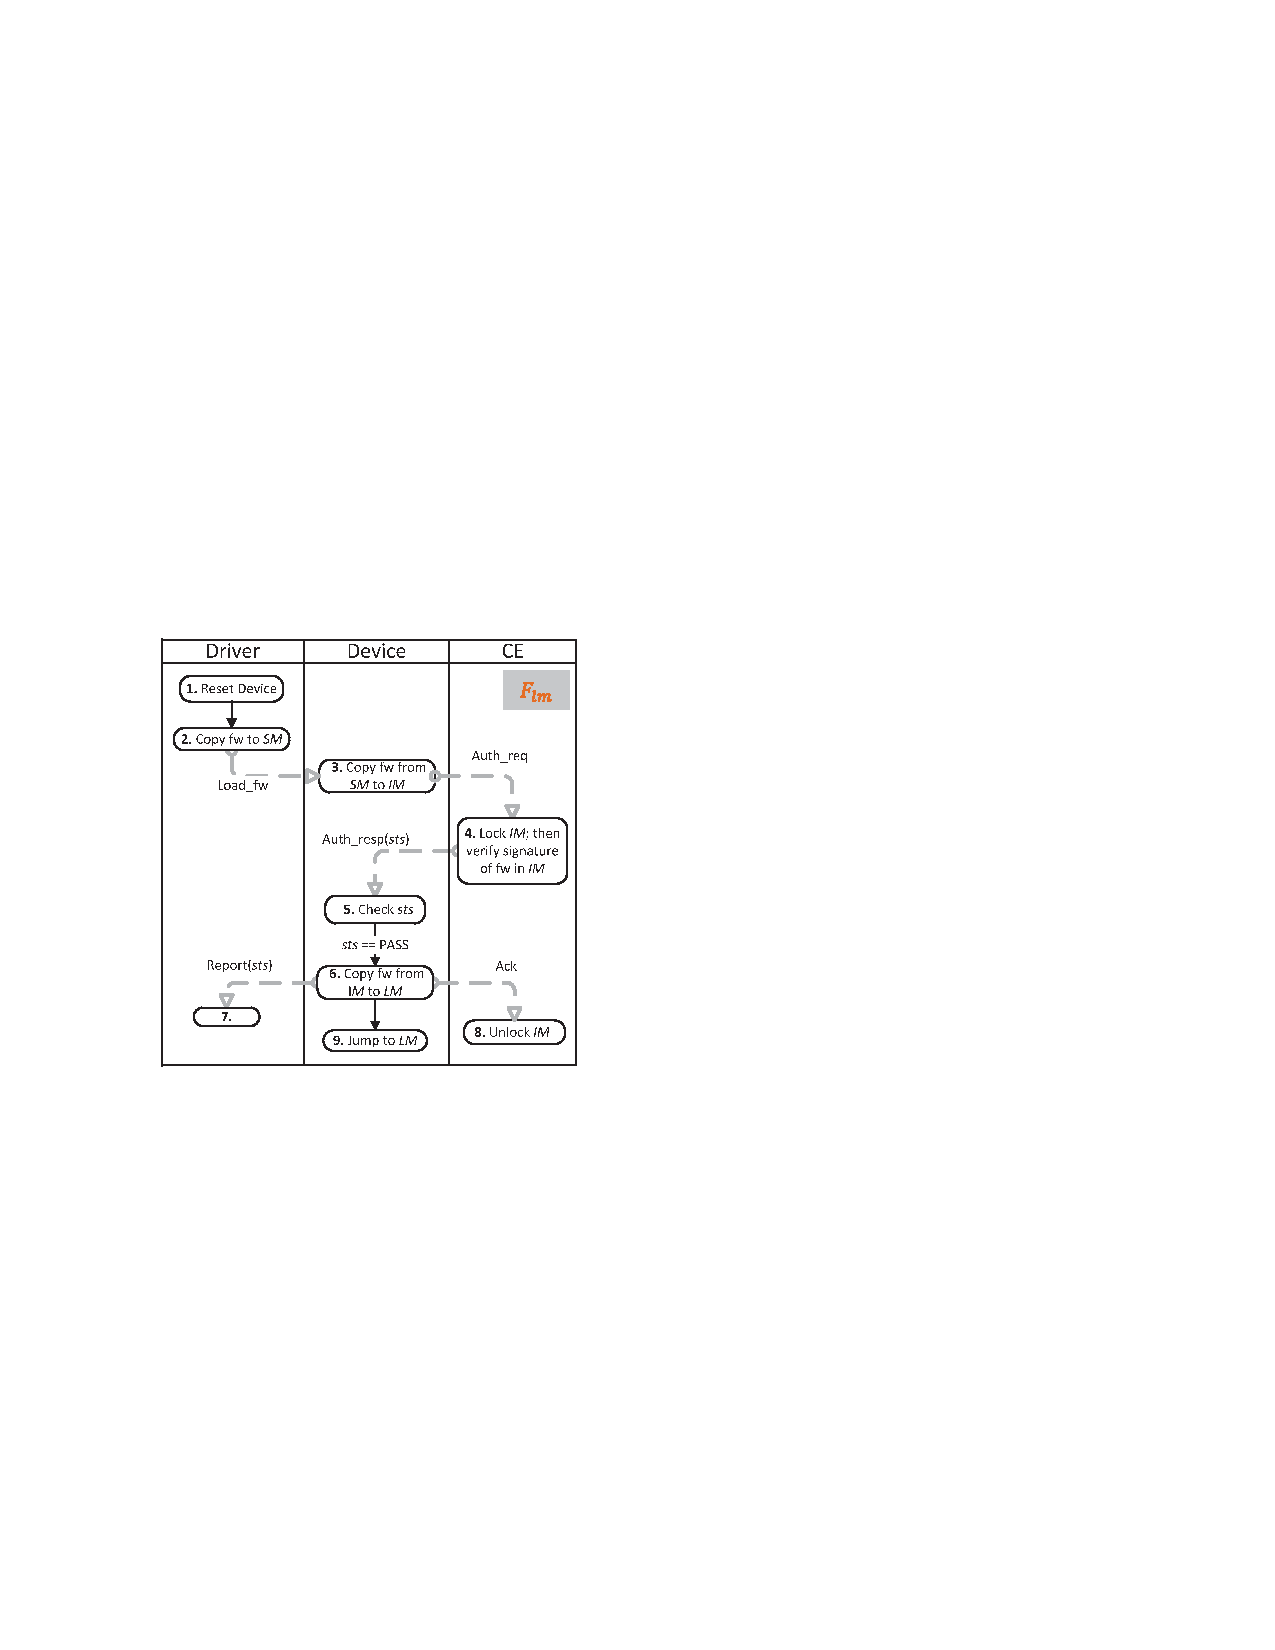
\includegraphics[height=2.5in]{figures/bpmn-flow-ex}
%% \caption{A graphical representation of a SoC firmware load protocol in BPMN~\cite{Krstic14HOST}.}
%% \label{flow-spec-ex}
%% \end{center}
%% \end{figure}
  
%% As indicated above, interpreting and understanding the raw signal traces observed from executing the chip is extremely difficult due to the limited observability and non-determinism.  This paper proposes a trace analysis method which analyzes and interprets the observed signal traces at the level of system flow specifications.  During the step of analysis and interpretation, this method tries to find out possible executions of system flows such that the observed signal trace is a result of such executions.  The resulting scenarios of flow executions often give debuggers more clear and better structured system-level views of the internal operations of the system under debug.  With a better understanding of system operations in a test environment, therefore, it would make easier for debuggers to pinpoint and root cause system failures.  In addition to debugging, another important benefit is better coverage evaluation as a scenario of flow executions captures the information about the types and number of instances of flows executed by the chip in a test environment.  That information can help to determine the quality and coverage of validation.   

%---

\begin{figure*}[tb]
\begin{center}
\begin{tabular}{cc}
\begin{minipage}{3in}
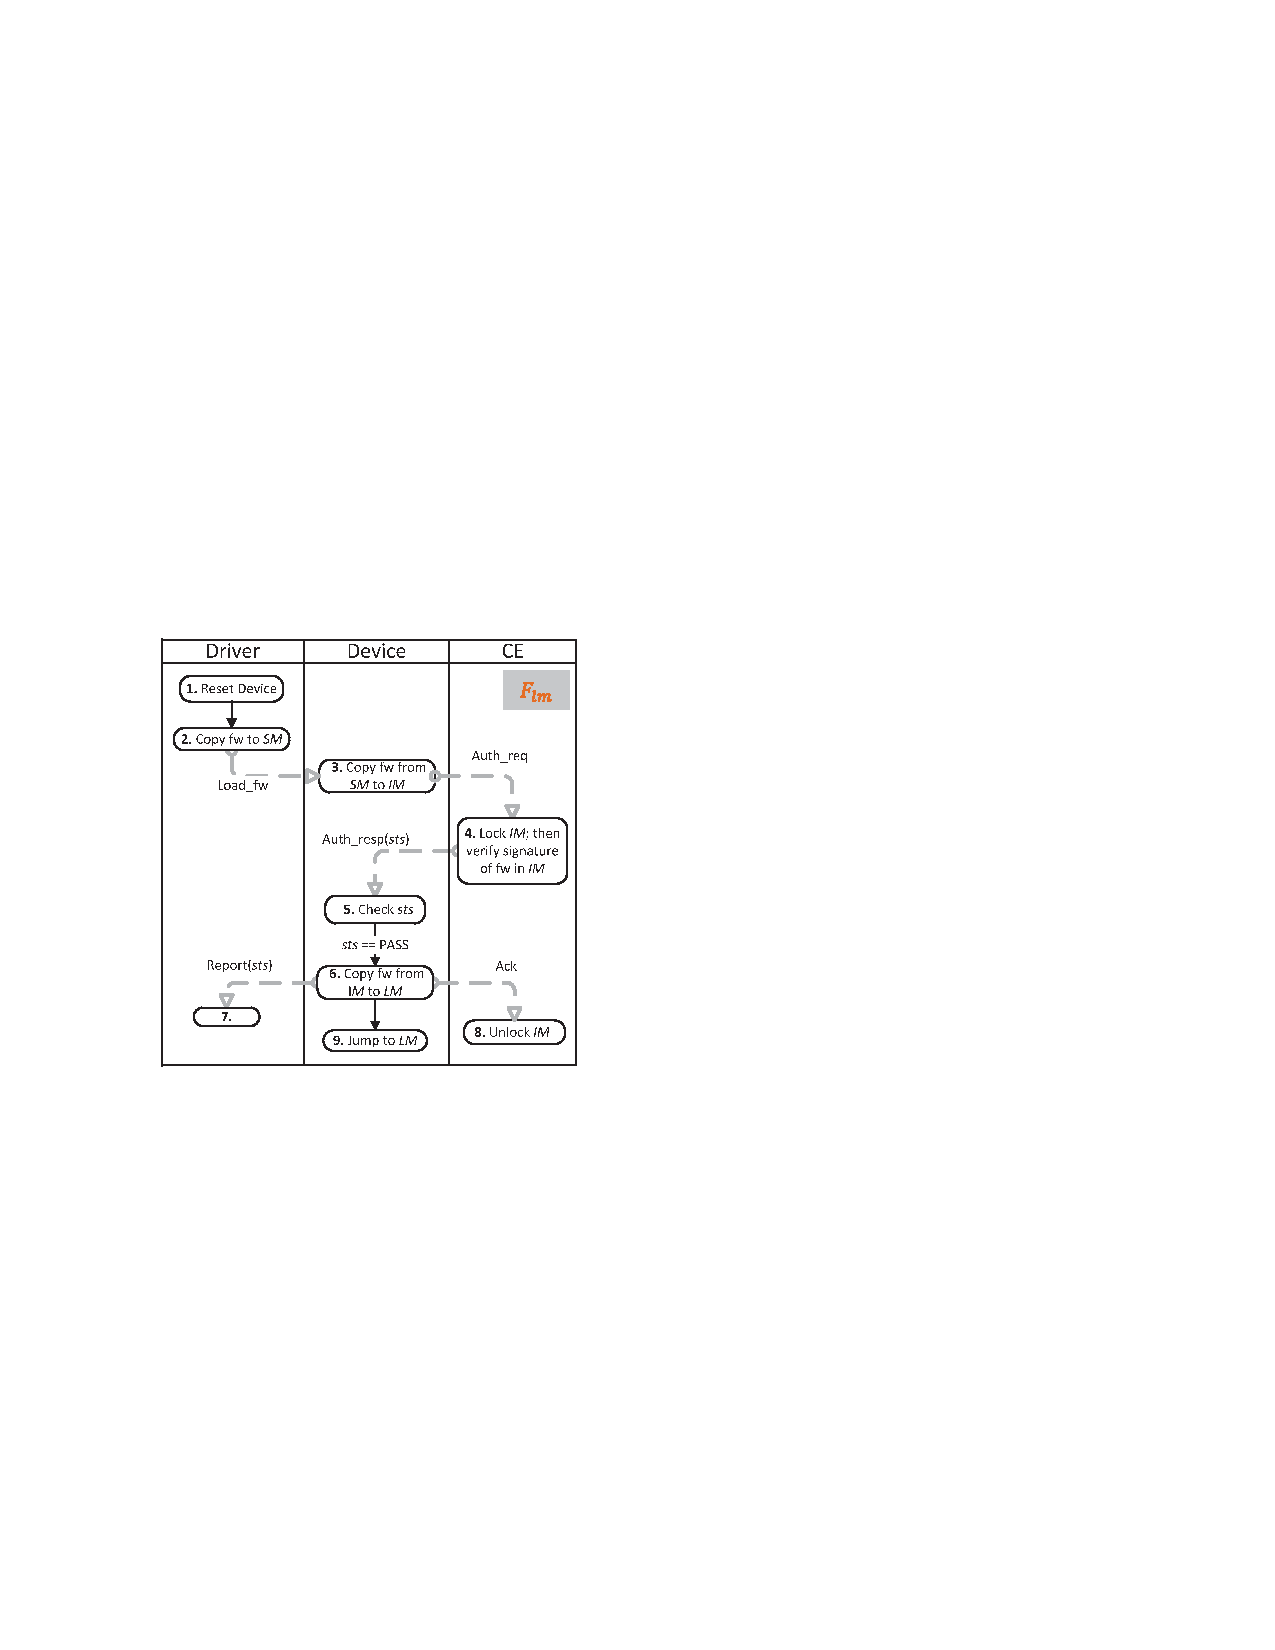
\includegraphics[height=2in]{figures/bpmn-flow-ex}
\end{minipage}
&
\begin{minipage}{3in}
\resizebox{2.8in}{!}{
\begin{tikzpicture}[node distance=3cm, auto,>=latex', thick]
\tikzset{rectbox/.style={rectangle, draw, align=flush center,thick, minimum size = 6mm}}
\tikzset{circ/.style={circle, draw,thick}}
\tikzset{terminal/.style={circle, draw,line width=.8mm}}
\tikzset{weight3/.style={line width=.3mm}}
	% Nodes:
	\node[circ]		(p1) 		at (0,0) {$p_1$};
	\node[rectbox]	(t1)	at	($(p1) + (0,-1.1)$) {$t_1:\langle {\tt Driver:Device:Load} \_fw\rangle$};
	\node[circ] 	(p2) 		at ($(t1) + (0,-1.1)$) {$p_2$};
	\node[rectbox]	(t2)	at	($(p2) + (0,-1.1)$) {$t_2:\langle {\tt Device:CE:Auth\_req} \rangle$};
	\node[circ] 	(p3) 		at ($(t2) + (0,-1.1)$) {$p_3$};
	\node[rectbox]	(t3)	at	($(p3) + (0,-1.1)$) {$t_3:\langle {\tt CE:Device:Auth\_resp}\rangle$};
	\node[circ] 	(p4) 		at ($(t3) + (0,-1.1)$) {$p_4$};
	\node[rectbox]	(t4)	at	($(p4) + (-3,-1.1)$) {$t_4:\langle {\tt Device:Driver:Report} \rangle$};
	\node[rectbox]	(t5)	at	($(p4) + (3,-1.1)$) {$t_5:\langle {\tt Device:CE:Ack} \rangle$};
	\node[circ,fill=black] 	(term1) 		at ($(t4) + (0,-1.1)$) {$~~~$};
	\node[circ,fill=black] 	(term2) 		at ($(t5) + (0,-1.1)$) {$~~~$};
	
	% Edges
	\draw[->,weight3]	(p1) -- (t1);
	\draw[->,weight3]	(t1) -- (p2);
	\draw[->,weight3]	(p2) -- (t2);
	\draw[->,weight3]	(t2) -- (p3);
	\draw[->,weight3]	(p3) -- (t3);
	\draw[->,weight3]	(t3) -- (p4);
	\draw[->,weight3]	(p4) -- ($(p4)+(-3,0)$) -- (t4);
	\draw[->,weight3]	(p4) -- ($(p4)+(3,0)$) -- (t5);
	\draw[->,weight3]	(t4) -- (term1);	
	\draw[->,weight3]	(t5) -- (term2);	
	
\end{tikzpicture}
}
\end{minipage}
\\
(a) & (b)
\end{tabular}
\caption{(a) A graphical representation of a SoC firmware
  load protocol~\cite{Krstic14HOST}.  (b) LPN formalization.
  Each event has a form of $\langle {\tt src, dest, cmd}
  \rangle$ where ${\tt cmd}$ is a command sent from a source
  component ${\tt src}$ to a destination component ${\tt
    dest}$. The solid black places without outgoing edges
  are {\em terminals}, which indicate termination of
  protocols represented by the LPNs.}
\label{flow-spec-ex}
\end{center}
\end{figure*}



\section{Labeled Petri-Nets}

Labeled Petri-nets (LPN) is a formalization of state
transition systems that is capable of describing sequencing,
concurrency, and choices.  Fig.~\ref{flow-spec-ex} shows the
formalization of a simple SoC protocol with Petri-Nets.
Formally, an LPN is a tuple $(P, T, s_0, E, L)$ where $P$ is
a finite set of {\em places}, $T$ is a finite set of {\em
  transitions}, $\mathit{init}$ is the set of initially
marked places, also referred to as the {\em initial
  marking}, $E$ is a finite set of {\em events}, and $L: T
\rightarrow E$ is a labeling function that maps each
transition $t \in T$ to an event $e \in E$.  For each
transition $t \in T$, its preset, denoted as $\bullet{t}
\subseteq P$, is the set of places connected to $t$, and its
postset, denoted as $t\bullet \subseteq P$, is the set of
places that $t$ is connected to.  A marking $s \subseteq P$
of a LPN is a subset of places marked with tokens, and it is
also referred to as a state of a LPN.  The initial marking
$\mathit{init}$ is also the initial state of the LPN.
  
%% This formalism has well defined
%% operational semantics, efficient analysis analysis
%% algorithms and and has been used widely in modeling and
%% analyzing communication protocols, concurrent programs, etc.

%--- LPN definition with levels
%Specifically, a labeled Petri-net (LPN) is a tuple $(P, T, M_0, V, E, L)$ where
%\begin{itemize}
%\item $P$ is a finite set of places,
%\item $T$ is a finite set of transitions,
%\item $M_0$ is the set of initially marked places, also referred to as the initial marking.
%\item $V$ is a finite set of auxiliary variables of integer type,
%\item $E$ is a finite set of events,
%\item $L$ is a labeling function that maps each transition $t \in T$ to a triple $(g, e, A)$ where
%	\begin{itemize}
%	\item $g$ is a predicate over $V$,
%	\item $e \in E$ is an event,
%	\item $A$ is a set of assignments to some variables in $V$.  
%	\end{itemize}
%\end{itemize}
%
%For each transition $t \in T$, its preset, denoted as $\bullet{t} \subseteq P$, is the set of places connected to $t$, and its postset, denoted as $t\bullet \subseteq P$, is the set of places that $t$ is connected to.  A marking of a LPN is a set of places marked with tokens, and a state of a LPN is $(M, \alpha)$ where $M$ is a marking and $\alpha$ is an assignment to all auxiliary variables in $V$.  
%
%The operational semantics of a LPN is defined by transition executions.  A transition can be executed after it is {\em enabled}.  A transition $t = (g, e, A)$ is enabled in a state $(M, \alpha)$ if every place in its preset is included in the marking, i.e. $\bullet{t} \subseteq M$, and the values of the auxiliary variables make the predicate $g$ be true, i.e. $\alpha \models g$.  Execution of $t$ results in a new state $(M', \alpha')$ such that 
%\[
%M' = (M - \bullet{t}) \cup t\bullet,
%\]
%and $\alpha'$ is a new assignment where the values of the auxiliary variables are updated with respect to the assignments $A$.  Furthermore, when $t$ is executed, the event $e$ is emitted.  SoC


%% Formally, an LPN is a tuple $(P, T, s_0, E, L)$ where $P$ is
%% a finite set of {\em places}, $T$ is a finite set of {\em
%%   transitions}, $\mathit{init}$ is the set of initially
%% marked places, also referred to as the {\em initial
%%   marking}, $E$ is a finite set of {\em events}, and $L: T
%% \rightarrow E$ is a labeling function that maps each
%% transition $t \in T$ to an event $e \in E$.  For each
%% transition $t \in T$, its preset, denoted as $\bullet{t}
%% \subseteq P$, is the set of places connected to $t$, and its
%% postset, denoted as $t\bullet \subseteq P$, is the set of
%% places that $t$ is connected to.  A marking $s \subseteq P$
%% of a LPN is a subset of places marked with tokens, and it is
%% also referred to as a state of a LPN.  The initial marking
%% $\mathit{init}$ is also the initial state of the LPN.

%% The operational semantics of a LPN is defined by transition executions.  A transition can be executed after it is {\em enabled}.  A transition $t \in T$ is enabled in a state $s$ if every place in its preset is included in the marking, i.e. $\bullet{t} \subseteq s$.  Execution of $t$ results in a new state $s'$ such that 
%% \[
%% s' = (s - \bullet{t}) \cup t\bullet,
%% \]
%% and the emission of event $e$ labeled for $t$. 

%% The communication protocol in the BMPN shown
%% in~Fig.~\ref{flow-spec-ex}(a) is represented by the LPN
%% shown in~Figure~\ref{flow-spec-ex}(b).  In this and the
%% following figures for LPNs, the labeled circles denote
%% places, and the labeled boxes denote transitions.  Each
%% transition is labeled with its name and the associated
%% event.  Each event has a form of $\langle {\tt src, dest,
%%   cmd} \rangle$ where ${\tt cmd}$ is a command sent from a
%% source component ${\tt src}$ to a destination component
%% ${\tt dest}$. The solid black places without outgoing edges
%% are {\em terminals}, which indicate termination of protocols
%% represented by the LPNs.  The initial marking is
%% $\mathit{init} = \{p_1\}$.  In this LPN model, only the
%% communication portion of the BPMN specification is
%% represented while the computation portion is ignored.




% @COMMENT This example is for LPNs with guards.
%The above protocol specification can be made more precise by describing how component~2 would respond without using non-determinism.  For example, the system architect may wish to specify that component~2  responds with $\mathit{msg_2}$ to every sequence of two $\mathit{msg_1}$ for five such sequences in a row.  On the sixth such sequence, component~2 responds with $\mathit{msg_3}$.  The LPN modeling such protocol is shown in Figure~\ref{fig-flow-ex-2}.  An alternative without using auxiliary variables in the transition predicates is by unrolling the loops for the specified number of times; however this would result in a larger and more complex LPN.  
%
%\begin{figure}[htbp]
%\begin{center}
%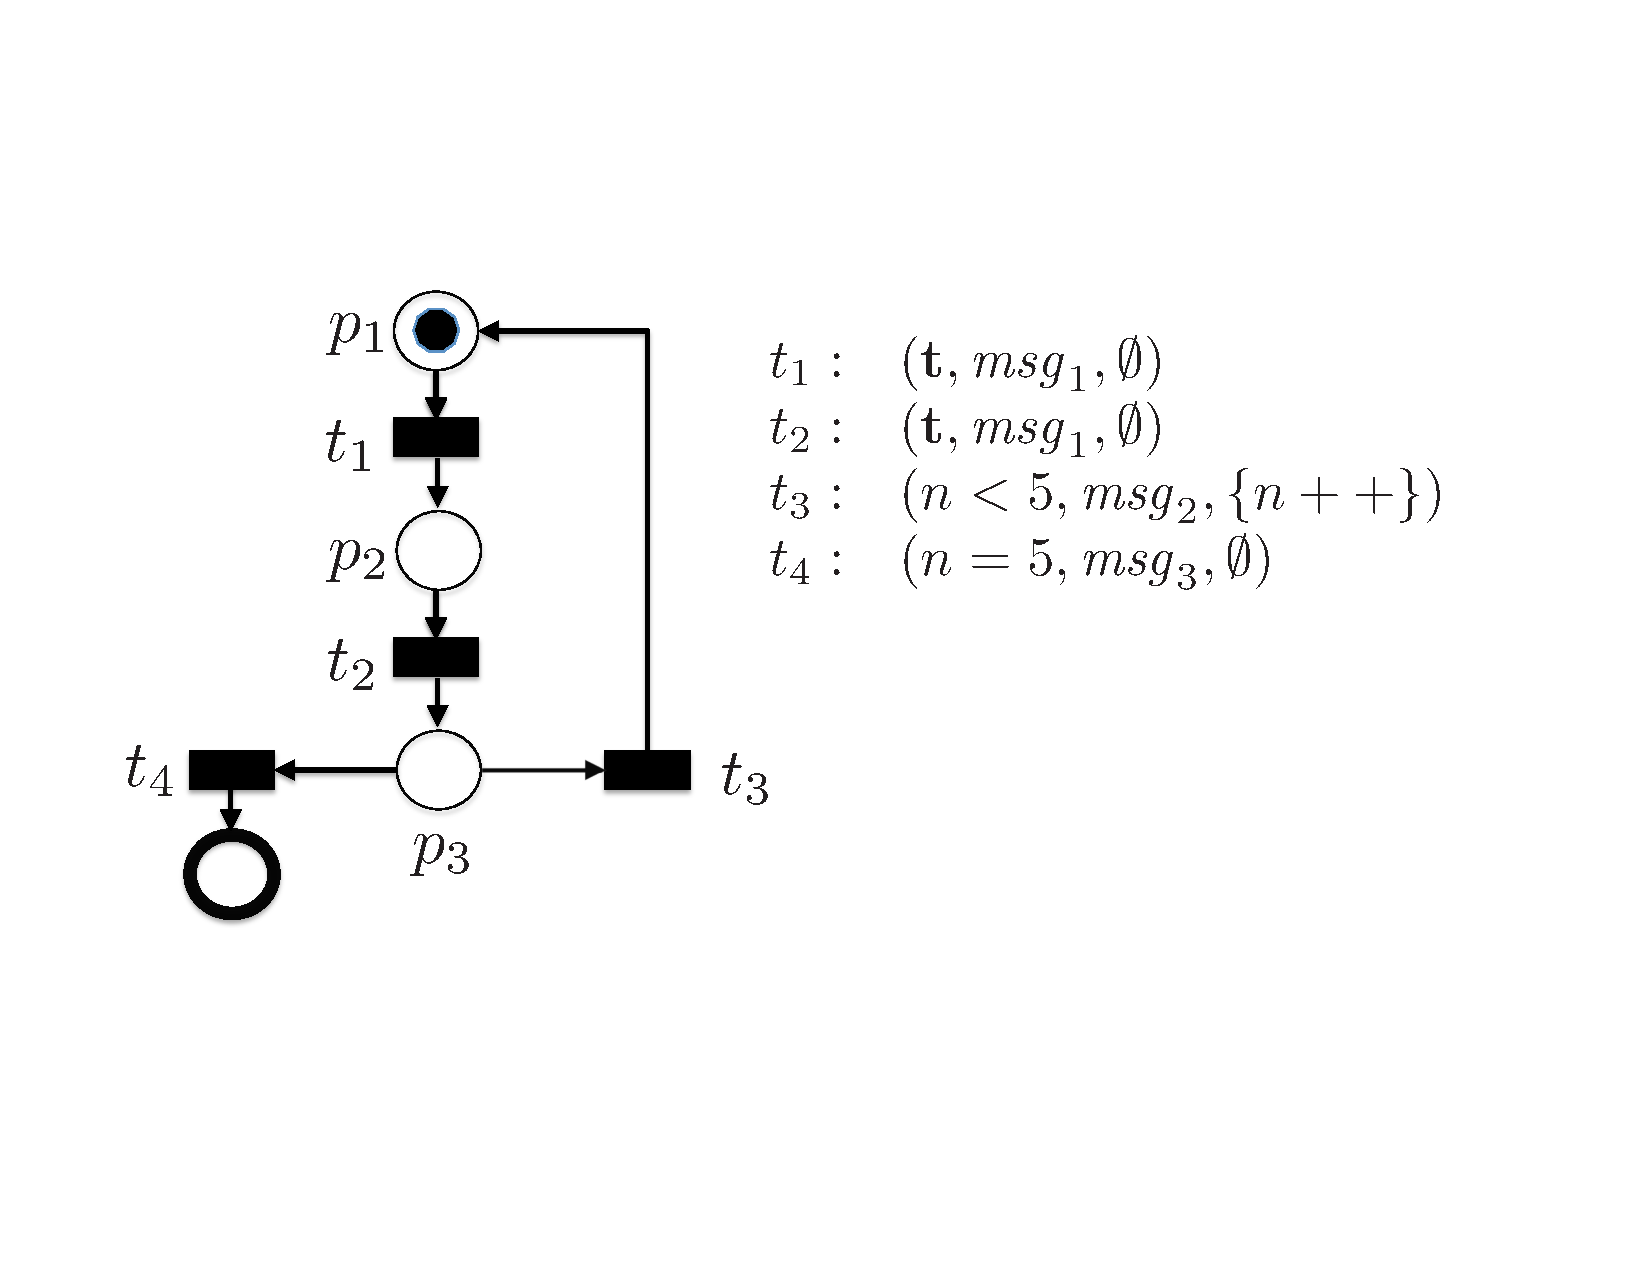
\includegraphics[height=1.6in]{figures/flow-ex-2}
%\caption{Another example of a LPN representing the system flow in Fig.~\ref{fig-flow-ex-1} with a fixed number of message exchanges.}
%\label{fig-flow-ex-2}
%\end{center}
%\end{figure}


%=====
\section{Flow-Directed Trace Analysis}

In a typical validation setting, the system under debug (SUD) is executed in a test environment until it is terminated by the test environment or the system crashes due to a failure.  During the execution, a trace on a small number of observable signals is streamed off the chip for debugging.  Due to the limited observability and inherent non-determinism in today's SoC designs, the observed signal trace is difficult to understand, thus providing limited values for debugging.  In this section, we describe a trace analysis method where the observed signal traces are interpreted at the level of system flows.  In general, the trace analysis can offer debuggers a structured view of communications among the IP blocks during the SUD execution by deriving the types and numbers of system flows activated during SUD executions from the observed signal traces.

The trace analysis method consists of two steps: \emph{trace abstraction} and \emph{interpretation}.  The trace abstraction takes a signal trace observed during the execution of the SUD, and abstracts it with respect to information captured in the system flows.  This requires recognizing signal events and mapping the signal events or sequences of the signal events to flow events appeared in system flow specifications.  For example, a data write message may be a single event in a system flow, however, such a flow event maybe implemented in hardware as a sequence of events including a header, a number of data word transfers and a tail.  This abstraction requires a mapping relation from flow events to sequences of signal events, and it is reasonable to assume that this relation is available.

The trace interpretation takes a finite trace of flow events resulting from the trace abstraction and a set of system flows in LPNs $\vec{F}$, and generates a set of possible system flow execution scenarios.  A \emph{flow execution scenario} is defined as $\{(F_{i,j}, s_{i,j})\}$ where in each element $(F_{i,j}, s_{i,j})$, $F_{i,j}$ is the $j$th activated instance of flow $F_i \in \vec{F}$, and $s_{i,j}$ is a state of $F_{i,j}$.  A flow execution scenario indicates that at a certain point of SUD execution, what types of flows and the number of instances of a particular flow are activated and their corresponding current states.

An observed trace of flow events $\rho = e_1e_2\ldots e_n$ is a result of SUD executing the flow instances of some flow execution scenario.  The goal of the trace interpretation is to derive such scenario.  Let $\mathit{accept(F_{i,j}, s_{i,j}, e)}$ be a function that determines if event $e$ can be emitted by $F_{i,j}$ in state $s_{i,j}$.  This function is used during the trace interpretation for checking whether an event of an observed trace is a result of executing some flow instance.  Formally,  $\mathit{accept(F_{i,j}, s_{i,j}, e)}$ returns $(F_{i,j}, s'_{i,j})$ if there exists a transition $t$ in $F_i$ such that $L(t) = e$ and $\bullet t \subseteq s_{i,j}$.  In this case, $s'_{i,j} = (s_{i,j} - \bullet t) \cup t\bullet$.  It returns $\emptyset$ if no such $t$ exists in $F_i$. 

Given a trace of flow events $\rho = e_1e_2\ldots e_n$, the trace interpretation algorithm starts with an empty set of of flow execution scenario $\mathit{Scen} = \emptyset$.  Then, for each $e_h$ where $1 \leq h \leq n$ starting $h=1$, and for each $\mathit{scen} \in \mathit{Scen}$, the following two steps are performed. 
\begin{description}
\item[Step 1]~~For each $(F_{i,j}, s_{i,j}) \in \mathit{scen}$, if $\mathit{accept}(F_{i,j}, s_{i,j}, e_h) = (F_{i,j}, s'_{i,j})$, create a new scenario $\mathit{scen}' = (\mathit{scen} - (F_{i,j}, s_{i,j})) \cup (F_{i,j}, s'_{i,j})$, which is added into $\mathit{Scen}'$.

\item[Step 2]~~For each $F_i \in \vec{F}$, create a new instance $F_{i, j+1}$.  If $\mathit{accept}(F_{i,j+1}, \mathit{init}_{i,j+1}, e_h) = (F_{i,j+1}, s'_{i,j+1})$,  create a new scenario $\mathit{scen}' = \mathit{scen} \cup (F_{i,j+1}, s'_{i,j+1})$, which is added into $\mathit{Scen}'$.
\end{description}
After $e_h$ is processed, $Scen = Scen'$, and the above two steps repeat for the next event $e_{h+1}$.

If every events in $\rho$ is successfully mapped to some flow instance, this algorithm returns a set of flow execution scenarios such that every flow instance is in its terminal state.  On the other hand, inconsistent events can also be encountered.  An event $e$ is \emph{inconsistent} if for each flow execution scenario $\mathit{scen} \in \mathit{Scen}$, the following two conditions hold.
\begin{enumerate}
\item For each $(F_{i,j}, s_{i,j}) \in \mathit{scen}$, $\mathit{accept}(F_{i,j}, s_{i,j}, e_h) = \emptyset$,
\item For each $F_i \in \vec{F}$, $\mathit{accept}(F_{i}, \mathit{init}_{i}, e_h) = \emptyset$.
\end{enumerate}
An inconsistent event is the one produced by SUD execution but cannot be mapped to any flow instances no matter how the trace prior to event $e$ is interpreted.  Inconsistent events indicates possible causes of system failures.     

Based on the above discussion, the trace interpretation algorithm returns two pieces of information: 1) a set $G$ of flow execution scenarios where every flow instance in every scenario is in its terminal state, 2) a set $B$ of pairs, each of which includes a set of flow execution scenarios and an inconsistent event.  The set $B$ provides valuable information for debuggers to root cause system failures.  One of these two sets can empty.   With the full observability, the set $G$ includes a single flow execution scenario derived for a trace.  In reality, it is always the case that the SUD is only partially observable.  Therefore, due to the lack of information for precise interpretation, a set of flow execution scenarios is typically derived for a given trace as the result of the trace analysis.    

\red{\bf The following illustration may not be needed (from here to the end of this subsection) if seciton IV is kept.  Or we keep the illustration below but remove section IV which uses 3 pages.}

To illustrate the basic idea of the trace analysis method, consider the system flow shown in Figure~\ref{fig-flow-ex-1}.  Let $F_1$ denote such flow.  Suppose that a hardware system implements flow $F_1$, and the following trace of flow events is abstracted from an observed signal trace as a result of executing such system.     
\[
\mathit{msg}_1\;\mathit{msg}_1\;\mathit{msg}_1\;\mathit{msg}_2\;\mathit{msg}_3\;\ldots
\]  
This trace is interpreted from the first event to the last in order to derive all possible flow execution scenarios.  At the beginning, the first event $\mathit{msg}_1$ is processed.  According to the flow specification $F_1$, we know that one instance of such flow $F_1$, $F_{1,1}$,  is activated by the SUD as $\mathit{accept}(F_{1,1}, init_1, \mathit{msg}_1) = (F_{1,1}, \{p_2\})$ where $\mathit{init} = \{p_1\}$ is the initial state of $F_1$.  As the result, the flow execution scenario after interpreting the first event $\mathit{msg_1}$ is $\{(F_{1,1}, \{p_2\})\}$.  

Next, the second $\mathit{msg}_1$ is interpreted on both scenarios   This event could be the result of two possible cases.  In the first case, this event is the result of the continuing execution of $F_{1,1}$ as $\mathit{accept}(F_{1,1}, \{p_2\}, \mathit{msg}_1) = (F_{1,1}, \{p_3\})$.  In the second case, the system may activate another instance of $F_1$, $F_{1,2}$ such that the second event $\mathit{msg_1}$ is a result of executing this new instance.  Therefore, the interpretation of the first two events $\mathit{msg}_1$ leads to two flow execution scenarios as shown below.
\[
\label{tr-analy-s1}\tag{1}
\begin{array}{cl}
1. & \{(F_{1,1}, \{p_3\})\},\\
2. & \{(F_{1,1}, \{p_2\}), (F_{1,2}, \{p_2\})\} 
\end{array}
\]

Now, consider the third $\mathit{msg}_1$ for each of the two scenario derived in~(\ref{tr-analy-s1}).    For the execution scenario~1, $F_{1,1}$ is not able to accept $\mathit{msg}_1$ as it is in state $\{p_3\}$.  On the other hand, this event could be the result of activation of a new flow instance.  Therefore, this execution scenario can be revised accordingly as 
\[
\label{tr-analy-s2}\tag{2}
\{(F_{1,1}, \{p_3\}),(F_{1,2},\{p_2\})\}.
\]   
For the execution scenario~2, event $\mathit{msg}_1$ could be the result of continuing execution of $F_{1,1}$ or $F_{1,2}$, or it could be a result of activation of a new flow instance.  Therefore,  three new execution scenarios can be derived as shown below for this event.
\[
\label{tr-analy-s3}\tag{3}
\begin{array}{l}
\{(F_{1,1}, \{p_3\}), (F_{1,2}, \{p_2\})\},\\
\{(F_{1,1}, \{p_2\}), (F_{1,2}, \{p_3\})\}, \\
\{(F_{1,1}, \{p_2\}), (F_{1,2}, \{p_2\}), (F_{1,3}, \{p_2\})\}
\end{array}
\]
Since the flow execution scenario in~(\ref{tr-analy-s2}) already exists in~(\ref{tr-analy-s3}), the three flow execution scenarios shown in~(\ref{tr-analy-s3}) is the result from the interpretation of the first three events $\mathit{msg}_1$.

The next flow event in the trace $\mathit{msg_2}$ is analyzed for the flow execution scenarios as shown in~(\ref{tr-analy-s3}).   For the first scenario $\{(F_{1,1}, \{p_3\}), (F_{1,2}, \{p_2\})\}$, event $\mathit{msg_2}$ can only be the result from executing $F_{1,1}$ as $\mathit{accept}(F_{1,1}, \{p_3\}, \mathit{msg_2}) = (F_{1,1}, \{p_1\})$.   Based on the same reasoning, this event can only be the result from executing $F_{1,2}$ in the second scenario, and it moves $F_{1,2}$ to a new state $\{p_3\}$ too.  The interesting case is the third scenario where none of the flow instances can allow $\mathit{msg_2}$ to happen.  This is due to the fact that the flow must be in $\{p_3\}$ for $\mathit{msg_2}$ to happen.  This indicates the third system execution scenario is impossible for the prefix of the flow event trace upto $\mathit{msg_2}$, therefore this scenario is ignored from further analysis.  After analyzing event $\mathit{msg_2}$, the updated system execution scenarios are shown below.
\[
\begin{array}{l}
\{(F_{1,1}, \{p_1\}), (F_{1,2}, \{p_2\})\},\ \{(F_{1,1}, \{p2\}), (F_{1,2}, \{p_1\})\}.
\end{array}
\]

The last flow event in the trace is $\mathit{msg}_3$.  Considering the above two possible system executions, neither can allow this event to be produced as none of the flow instances in both system executions is in state $\{p_3\}$.  What this means is that the system does {\em not} implement the flow specification correctly as it produces something not allowed by the specification.  By examining the system executions right before the ``buggy'' event, debuggers may gain more information on when and where the problem might be.  The trace interpretation algorithm adds these two scenarios along with the fifth event $\mathit{msg_3}$ into $B$, and returns it for debuggers to analyze.



%---
\subsection{Trace Analysis with Partial Observability}

In hardware that implements a given system flow specification, a flow event is defined as an event or a sequence of events on a set of signals.  Due to the limited number of pins on the boundary of chips available for observation, only a small fraction of system signals can be observed during debug.  In this section, we discuss how the trace analysis method presented above can be adapted to deal with signal traces of partial observability.

In general, a signal trace of partial observability corresponding a set of traces of flow events due to the ambiguous interpretation of signal events.  In the following, we discuss two cases for trace abstraction on partial observability: mapping a single signal event to a flow event or mapping a sequence of signal events to a flow event.  A signal event is defined as a state on or an assignment to a set of signals.  

Hereafter, the term {\em flow traces} is used to refer to traces of flow events. 
Consider the following example for the first case.  Suppose that there are three flow events: $e_1$, $e_2$, and $e_3$, which are implemented in hardware by the signal events shown in the list below.  We use Boolean expressions to represent signal events for the discussion.
\[
\begin{array}{cl}
e_1: & abc\\
e_2: & \bar{a}bc\\
e_3: & a\bar{b}c
\end{array}
\] 
Now suppose that only signals $b$ and $c$ are observable, and a signal trace of this partial observability is obtained below.
\[
bc\ bc \ \bar{b}c
\]
During the trace abstraction step, the first two signal events $bc$ can be mapped to $\{e_1, e_2\}$ since $a$ is not observable, and the last one $b'c$ is mapped to $\{e_3\}$.  Therefore, this signal trace is abstracted to four flow traces, $\{e_1, e_2\} \times \{e_1, e_2\} \times \{e_3\}$.

Next, we consider the case where a flow event is mapped from a sequence of signal events.  Now suppose that two other flow events are implemented by sequences of signal events as defined in the list below.
\[
\begin{array}{cl}
e_4: & abc\ \bar{a}bc\\
e_5: & abc\ abc\ abc\ \bar{a}bc\\
\end{array}
\] 
Given an observed trace of the same observability shown below
\[
bc\ bc\ bc \ bc,
\]
it is abstracted to the following flow traces.
\[
e_4e_4,\; \textvisiblespace e_4 \textvisiblespace,\;  e_4 \textvisiblespace \textvisiblespace,\;  \textvisiblespace \textvisiblespace e_4, \; e_5
\] 
where $\textvisiblespace$ denotes signal events that are not mapped to any flow events.  Note that the above abstraction leads to three distinct flow traces as the middle three correspond to the same trace of flow events. 


From the above discussions, it can be seen that a signal trace of partial observability is generally mapped to a set of flow traces.  As the the number of signals available for observation becomes smaller, the number of flow event traces corresponding to a signal trace as a result of the abstraction can be enormous.  This phenomenon can increase the complexity of the trace interpretation as it can cause the number of possible flow execution scenarios generated during the analysis to explode.   Possible solutions to address this issue include better trace signal selection for observation and assistance from debuggers' insights.  Trace signal selection itself is an important and difficult subject, and a detailed discussion of it is out of scope of this paper.   Next, we briefly describe how the debuggers' insights of a system's architecture can help to address the complexity issue in the trace analysis.


\subsection{Inputs from Validators}

During the trace interpretation, the number of intermediate flow execution scenarios may become too large due to ambiguous interpretation from signal events to flow events or from flow events to flow execution scenarios.  The explosion of the intermediate results can significantly slow down the performance of the trace analysis.  To address this problem, the debuggers can use their insights and understanding of the SUD to trim the total number of possible system executions derived from the trace analysis.  When a SUD is validated, a debugger is assumed to have deep knowledge about the system's architecture and microarchitecture, and how the test environment affects the system executions.  For instance, he/she may have knowledge that in a test environment, the maximal number of instances of a flow can be activated by the SUD, or a flow can be activated after certain other flows have terminated, etc.  These debugging insights can be encoded as constraints into the trace analysis method, which can then be used to eliminate a large number of flow execution scenarios that violate these constraints during the trace interpretation step.

This approach can be flexible in that it allows a debugger to analyze the observed traces in a trail-and-error manner if the precise knowledge of the system (micro-)architecture is hard to come by.  For instance, the debugger might initially make a very restricted assumption on how the SUD executes a flow specification, and these assumptions can potentially lead to an empty set of flow execution scenarios.  Depending on which of these assumptions triggered during the trace interpretation step, the debugger can study these assumptions more carefully, and relax some or all of them for the next run of analysis.  This iteration can be repeated as many times as necessary until some results deemed meaningful are produced.

Alternatively, if all derived execution scenarios seem to be plausible, the implication that a debugger may draw from this result is that the failure may be independent of the flows being observed.  Therefore, the testing environment can be adjusted in order for a different part or different behavior of the SUD to be observed.  This idea, closely related to trace signal selection, is critical for post-silicon validation, and a detailed discussion can only be presented in a separate paper. 


  

%=====
\section{Case Study}

The proof concept of the proposed trace analysis method is demonstrated on a transaction level model of a simple SoC design with two CPU cores, memory, and a peripheral device connected by an interconnect as shown in Fig.~\ref{fig-SoC-ex}.  Since the analysis method presented in this paper is communication centric, the detailed computations of these blocks are not modeled.  Instead, the modeling is focused on how they participate in flows for different system level use cases.

\begin{figure}[tb]
\begin{center}
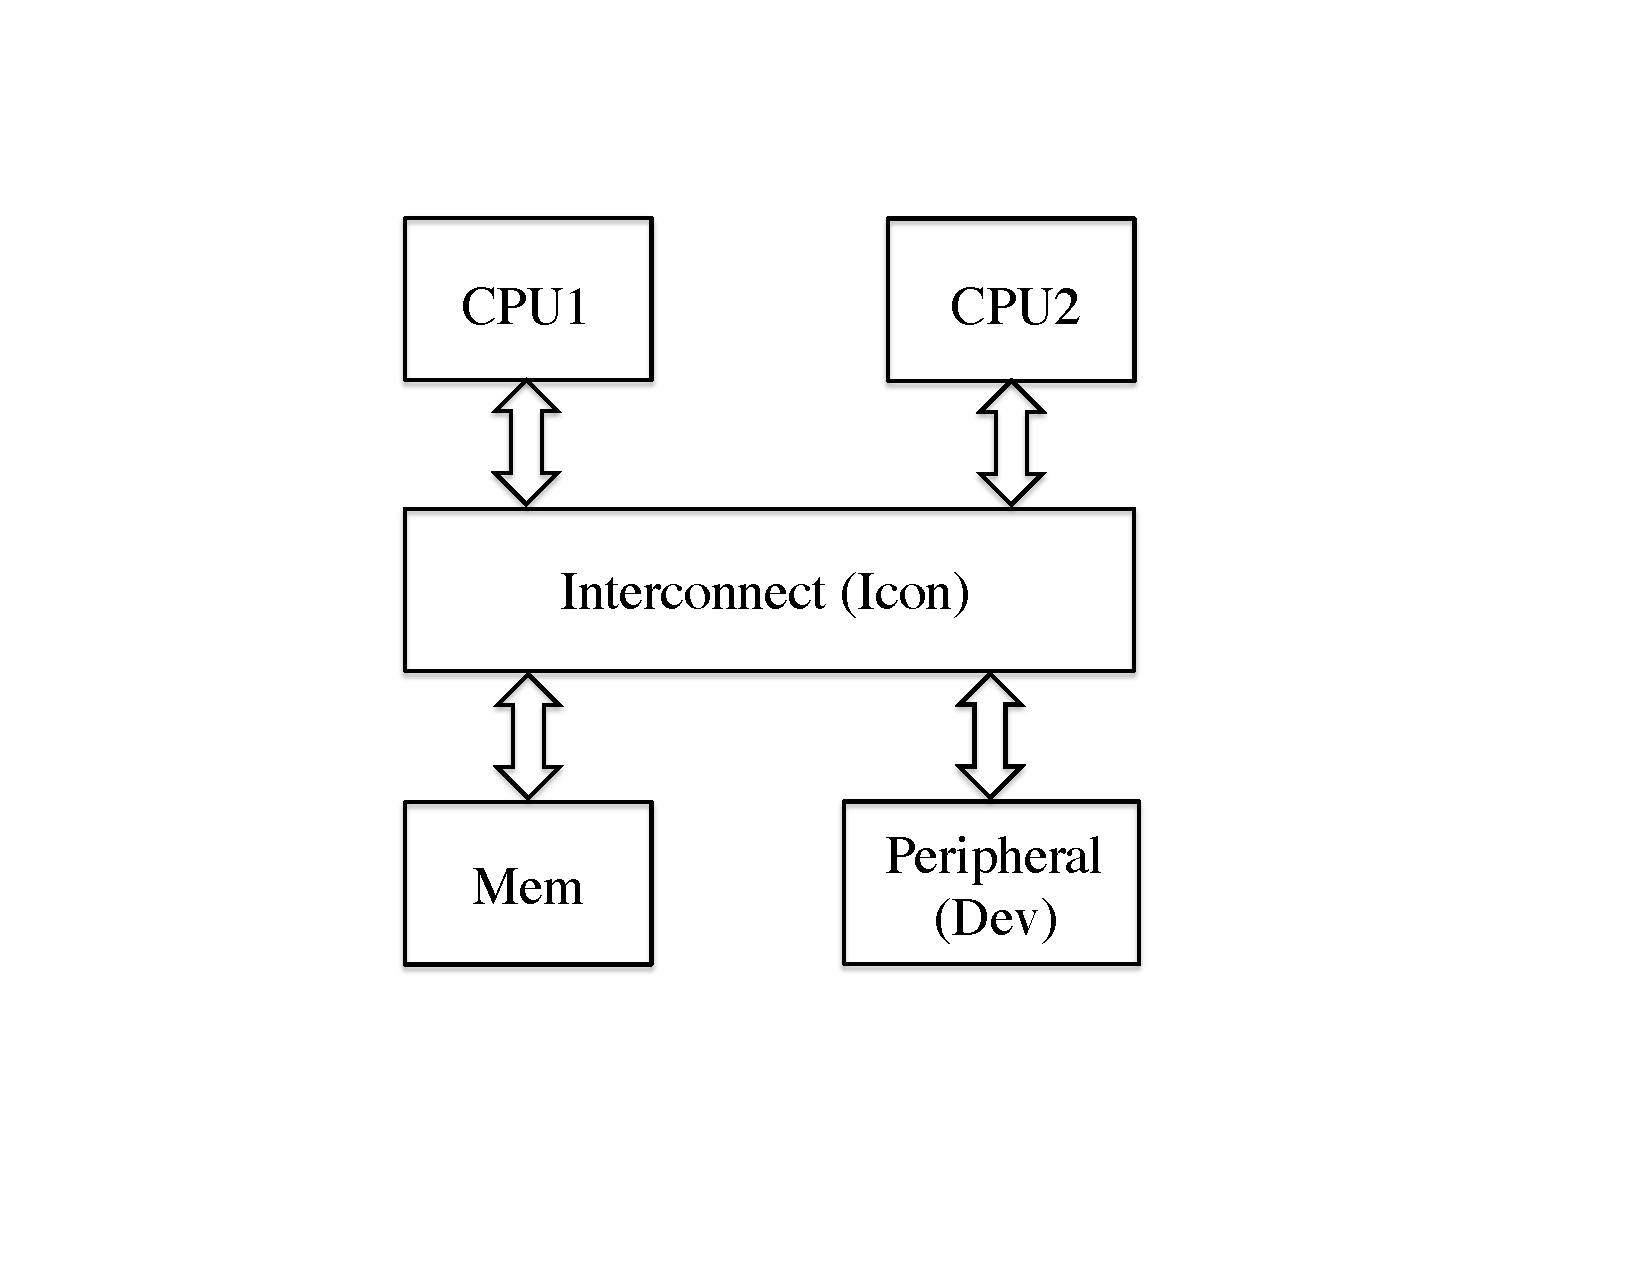
\includegraphics[width=2in]{figures/simple-ex}
\caption{A simple SoC example.}
\label{fig-SoC-ex}
\end{center}
\end{figure}


\subsection{Flow Specification}

In this case study, four system flows are implemented in the simple SoC model. They include cache coherent memory access operations and a memory-mapped peripheral read operation initiated from the CPUs, a message signaled interrupt operation initiated from the peripheral device.  These flow specifications capture how messages are exchanged for different use cases.  In this model, a message is defined with the following format, $(\mbox{Src}, \mbox{Dest}, \mathit{Cmd}, \mathit{Addr})$, where Src and Dest refer to the source and destination components of messages, $\mathit{Cmd}$ refers to the operations that the destination component should perform, and $\mathit{Addr}$ refers to memory addresses where $\mathit{Cmd}$ applies.  $\mathit{Cmd}$ can be memory accesses or not.  If it is not, then the $\mathit{Addr}$ field of messages is ignored.  In this case study, memory mapped IO mechanism is used.  Furthermore, detailed memory addresses are not modeled. Instead, the address space is partitioned to main memory addresses and peripheral addresses.  In messages, the $\mathit{Addr}$ field is replaced with either $M$ representing a memory address or $P$ representing an address to a peripheral device.  

The LPN as shown in Fig.~\ref{fig-cpu-write} specifies a system flow where {CPU2} initiates a memory write operation.   In this flow, CPU2 initiates a memory write request followed by a data valid message to the interconnect.  The data valid messages are used to model availability or validity of data for transfer.  Concurrently, the interconnect inquiries CPU1 if it holds a more updated version of the data by sending a memory write message $\mathit{msg_2}$.   CPU1 generates one of two possible responses.  If CPU1 holds the more updated data in its cache in the same memory space that CPU2 intends to write, a cache hit message $\mathit{msg_4}$ followed by $\mathit{msg_6}$ are sent to the interconnect.  Otherwise, CPU1 sends a cache miss message $\mathit{msg_5}$.  After getting the response from CPU1, Interconnect sends a write request to the memory unit.  This flow is symmetric for CPU1.

\begin{figure}[tb]
\begin{center}
\resizebox{2.8in}{!}{
\begin{tikzpicture}[node distance=3cm, auto,>=latex', thick]
\tikzset{rectbox/.style={rectangle, draw, align=flush center,thick, minimum size = 6mm}}
\tikzset{circ/.style={circle, draw,thick}}
\tikzset{terminal/.style={circle, draw,line width=.8mm}}
\tikzset{weight3/.style={line width=.3mm}}
	% Nodes:
	\node[circ]		(p1) 		at (0,0) {$p_1$};
	\node[rectbox]	(msg1)	at	($(p1) + (0,-1.1)$) {$msg_1$};
	\node[circ] 	(p2) 		at ($(msg1) + (-3,0)$) {$p_2$};
	\node[circ] 	(p3) 		at ($(msg1) + (3,0)$) {$p_3$};
	\node[rectbox]	(msg2)	at	($(p2) + (0,-1.1)$) {$msg_2$};
	\node[rectbox]	(msg3)	at	($(p3) + (0,-1.5)$) {$msg_3$};
	\node[circ] 	(p4) 		at ($(msg2) + (0,-1.1)$) {$p_4$};
	\node[rectbox]	(msg4)	at	($(p4) + (0,-1.1)$) {$msg_4$};
	\node[rectbox]	(msg5)	at	($(p4) + (3,0)$) {$msg_5$};
	\node[circ] 	(p6) 		at ($(msg4) + (0,-1.1)$) {$p_6$};
	\node[circ] 	(p5) 		at ($(msg3) + (0,-1.4)$) {$p_5$};
	\node[rectbox,rotate=90]	(msg6)	at	($(p6) + (1.5,0)$) {$msg_6$};
	\node[circ] 	(p7) 		at ($(msg6) + (1.5,0)$) {$p_7$};
	\node[rectbox]	(msg7)	at	($(p5) + (0,-1.5)$) {$msg_7$};
	\node[terminal]	(p8)	at	($(msg7) + (2,0)$) {$p_8$};
	% Edges
	\draw[->,weight3]	(p1) -- (msg1);
	\draw[->,weight3]	(msg1) -- (p2);
	\draw[->,weight3]	(msg1) -- (p3);
	\draw[->,weight3]	(p2) -- (msg2);
	\draw[->,weight3]	(msg2) -- (p4);
	\draw[->,weight3]	(p4) -- (msg4);
	\draw[->,weight3]	(p4) -- (msg5);
	\draw[->,weight3]	(msg4) -- (p6);
	\draw[->,weight3]	(p6) -- (msg6);
	\draw[->,weight3]	(msg6) -- (p7);
	\draw[->,weight3]	(p7) -- (msg7);
	\draw[->,weight3]	(msg7) -- (p8);
	\draw[->,weight3]	(msg5) -- (p7);
	\draw[->,weight3]	(p3) -- (msg3);
	\draw[->,weight3]	(msg3) -- (p5);
	\draw[->,weight3]	(p5) -- (msg7);
	
	\node[]	(msg-def)	at	($(p1) + (0,-8.5)$) {
	\begin{minipage}{3in}
	Definition of the messages:
\[
\begin{array}{clllll}
msg_1: & (\mbox{CPU2},	& \mbox{Icon},		& \mathit{Wr}, 	& M) \\
msg_2: & (\mbox{Icon},	& \mbox{CPU1}, 	& \mathit{Wr},			& M) \\
msg_3: & (\mbox{CPU2},	& \mbox{Icon}, 	& \mathit{DVal},	& -) \\
msg_4: & (\mbox{CPU1},	& \mbox{Icon}, 	& \mathit{Hit},	& -) \\
msg_5: & (\mbox{CPU1},	& \mbox{Icon}, 	& \mathit{Miss},	& -) \\
msg_6: & (\mbox{CPU1},	& \mbox{Icon}, 	& \mathit{DVal},	& -) \\
msg_7: & (\mbox{Icon},	& \mbox{Mem}, 		& \mathit{Wr},			& M) \\
\end{array}
\]
\end{minipage}
		};
\end{tikzpicture}
}
\caption{Flow specification ($F_1$) of a cache coherent write operation initiated from \texttt{CPU2}.}
\label{fig-cpu-write}
\end{center}
\end{figure}


The LPN specification as shown in Fig.~\ref{fig-cpu-read} captures the system flow where CPU2 initiates a memory read operation.  Basically, CPU2 sends a memory read message to Interconnect, which then generates two concurrent threads, one checks if CPU1 has the more updated data in the memory space for the read operation, and the other thread to get data from the memory.  Once Interconnect gets both responses from CPU1 and memory, it synchronizes the responses, and writes the correct data to the CPU2's cache and memory in parallel.  Again, this specification is symmetric for CPU1.


\begin{figure}[htbp]
\begin{center}
\resizebox{3.2in}{!}{
\begin{tikzpicture}[node distance=3cm, auto,>=latex', thick]
\tikzset{rectbox/.style={rectangle, draw, align=flush center,thick, minimum size = 6mm}}
\tikzset{circ/.style={circle, draw,thick}}
\tikzset{terminal/.style={circle, draw,line width=.8mm}}
\tikzset{weight3/.style={line width=.3mm}}
	% Nodes:
	\node[circ]		(p1) 		at (0,0) {$p_1$};
	\node[rectbox]	(msg1)	at	($(p1) + (0,-1.1)$) {$msg_1$};
	\node[circ] 	(p2) 		at ($(msg1) + (-3,0)$) {$p_2$};
	\node[circ] 	(p3) 		at ($(msg1) + (2,0)$) {$p_3$};
	\node[rectbox]	(msg2)	at	($(p2) + (0,-1.1)$) {$msg_2$};
	\node[rectbox]	(msg3)	at	($(p3) + (2,0)$) {$msg_3$};
	\node[circ] 	(p4) 		at ($(msg2) + (0,-1.1)$) {$p_4$};
	\node[rectbox]	(msg4)	at	($(p4) + (0,-1.1)$) {$msg_4$};
	\node[rectbox]	(msg5)	at	($(p4) + (3,0)$) {$msg_5$};
	\node[circ] 	(p6) 		at ($(msg4) + (0,-1.1)$) {$p_6$};
	\node[circ] 	(p5) 		at ($(msg3) + (0,-1.1)$) {$p_5$};
	\node[rectbox,rotate=90]	(msg6)	at	($(p6) + (1.5,0)$) {$msg_6$};
	\node[circ] 	(p7) 		at ($(msg6) + (1.5,0)$) {$p_7$};
	\node[rectbox]	(msg7)	at	($(p5) + (0,-1.1)$) {$msg_7$};
	\node[circ]	(p8)	at	($(msg7) + (0,-1.1)$) {$p_8$};
	\node[rectbox]	(msg8)	at	($(p8) + (0,-1.1)$) {$msg_8$};
	\node[circ]	(p9)	at	($(msg8) + (-1.5,-1.1)$) {$p_9$};
	\node[circ]	(p10)	at	($(msg8) + (1.5,-1.1)$) {$p_{10}$};
	\node[rectbox]	(msg9)	at	($(p9) + (0,-1.1)$) {$msg_9$};
	\node[rectbox]	(msg10)	at	($(p10) + (0,-1.1)$) {$msg_{10}$};
	\node[terminal]	(p11)	at	($(msg9) + (0,-1.1)$) {$p_{11}$};
	\node[terminal]	(p12)	at	($(msg10) + (0,-1.1)$) {$p_{12}$};

	% Edges
	\draw[->,weight3]	(p1) -- (msg1);
	\draw[->,weight3]	(msg1) -- (p2);
	\draw[->,weight3]	(msg1) -- (p3);
	\draw[->,weight3]	(p2) -- (msg2);
	\draw[->,weight3]	(msg2) -- (p4);
	\draw[->,weight3]	(p4) -- (msg4);
	\draw[->,weight3]	(p4) -- (msg5);
	\draw[->,weight3]	(msg4) -- (p6);
	\draw[->,weight3]	(p6) -- (msg6);
	\draw[->,weight3]	(msg6) -- (p7);
	\draw[->,weight3]	(p7) -- (msg8);
	\draw[->,weight3]	(msg7) -- (p8);
	\draw[->,weight3]	(msg5) -- (p7);
	\draw[->,weight3]	(p3) -- (msg3);
	\draw[->,weight3]	(msg3) -- (p5);
	\draw[->,weight3]	(p5) -- (msg7);
	\draw[->,weight3]	(p8) -- (msg8);
	\draw[->,weight3]	(msg8) -- (p9);
	\draw[->,weight3]	(msg8) -- (p10);
	\draw[->,weight3]	(p9)  -- (msg9);
	\draw[->,weight3]	(p10)  -- (msg10);
	\draw[->,weight3]	(msg9) -- (p11);
	\draw[->,weight3]	(msg10) -- (p12);
	
	\node[]	(msg-def)	at	($(p1) + (-2.7,-10)$) {
	\begin{minipage}{2in}
	Definition of the messages:
\[
\begin{array}{clllll}
msg_1: & (\mbox{CPU2},	& \mbox{Icon},		& \mathit{Rd}, 		& M) \\
msg_2: & (\mbox{Icon},	& \mbox{CPU1}, 	& \mathit{Rd},	& M) \\
msg_3: & (\mbox{Icon},	& \mbox{Mem}, 		& \mathit{Rd},			& M) \\
msg_4: & (\mbox{CPU1},	& \mbox{Icon}, 	& \mathit{Hit},	& -) \\
msg_5: & (\mbox{CPU1},	& \mbox{Icon}, 	& \mathit{Miss},& -) \\
msg_6: & (\mbox{CPU1},	& \mbox{Icon}, 	& \mathit{DVal},	& -) \\
msg_7: & (\mbox{Mem},		& \mbox{Icon}, & \mathit{DVal},			& -) \\
msg_8: & (-,		& -, 		& -,				& -) \\
msg_9: & (\mbox{Icon},	& \mbox{Mem}, 		& \mathit{Wr},			& M) \\
msg_{10}: & (\mbox{Icon},	& \mbox{CPU2}, 		& \mathit{Wr},			& M) \\
\end{array}
\]
\end{minipage}
		};

\end{tikzpicture}
}
\caption{Flow specification ($F_2$) of a cache coherent read operation from CPU2.}
\label{fig-cpu-read}
\end{center}
\end{figure}


The LPN specification as shown in Fig.~\ref{fig-peri-read} captures a system flow for CPU initiated memory mapped peripheral read operations.  When CPU2 tries to read the peripheral device (device hereafter), a read message with address $P$ is sent to Interconnect, which then sends this message to CPU1 and the device simultaneously.  When CPU1 sees this message, it responds with a cache miss message as the address $P$ points to the device.  At the meantime, the device responds with a data valid message indicating the availability of the requested data.  Finally, Interconnect synchronizes the both responses, and sends a data valid message back to CPU2.   This specification is also symmetric for CPU1.

\begin{figure}[tb]
\begin{center}
\resizebox{3.2in}{!}{
\begin{tikzpicture}[node distance=3cm, auto,>=latex', thick]
\tikzset{rectbox/.style={rectangle, draw, align=flush center,thick, minimum size = 6mm}}
\tikzset{circ/.style={circle, draw,thick}}
\tikzset{terminal/.style={circle, draw,line width=.8mm}}
\tikzset{weight3/.style={line width=.3mm}}
	% Nodes:
	\node[circ]		(p1) 		at (0,0) {$p_1$};
	\node[rectbox]	(msg1)	at	($(p1) + (0,-1.1)$) {$msg_1$};
	\node[circ] 	(p2) 		at ($(msg1) + (-1.5,0)$) {$p_2$};
	\node[circ] 	(p3) 		at ($(msg1) + (1.5,0)$) {$p_3$};
	\node[rectbox]	(msg2)	at	($(p2) + (-1.5,0)$) {$msg_2$};
	\node[rectbox]	(msg4)	at	($(p3) + (1.5,0)$) {$msg_4$};
	\node[circ] 	(p4) 		at ($(msg2) + (-1.5,0)$) {$p_4$};
	\node[rectbox]	(msg3)	at	($(p4) + (0,-1.2)$) {$msg_3$};
	\node[circ] 	(p6) 		at ($(msg3) + (0,-1.2)$) {$p_6$};
	\node[circ] 	(p5) 		at ($(msg4) + (1.5,0)$) {$p_5$};
	\node[rectbox]	(msg5)	at	($(p5) + (0,-1.2)$) {$msg_5$};
	\node[circ]	(p7)	at	($(msg5) + (0,-1.2)$) {$p_7$};
	\node[rectbox]	(msg6)	at	($(p6) + (4.5,0)$) {$msg_6$};
	\node[terminal]	(p8)	at	($(msg6) + (0,-1.2)$) {$p_8$};

	% Edges
	\draw[->,weight3]	(p1) -- (msg1);
	\draw[->,weight3]	(msg1) -- (p2);
	\draw[->,weight3]	(msg1) -- (p3);
	\draw[->,weight3]	(p2) -- (msg2);
	\draw[->,weight3]	(msg2) -- (p4);
	\draw[->,weight3]	(p4) -- (msg3);
	\draw[->,weight3]	(msg3) -- (p6);
	\draw[->,weight3]	(p6) -- (msg6);
	\draw[->,weight3]	(msg6) -- (p8);
	\draw[->,weight3]	(p3) -- (msg4);
	\draw[->,weight3]	(msg4) -- (p5);
	\draw[->,weight3]	(p5) -- (msg5);
	\draw[->,weight3]	(msg5) -- (p7);
	\draw[->,weight3]	(p7) -- (msg6);
	\draw[->,weight3]	(msg6) -- (p8);
	
		\node[]	(msg-def)	at	($(p8) + (0,-2.5)$) {
	\begin{minipage}{3in}
	Definition of the messages:
\[
\begin{array}{clllll}
msg_1: & (\mbox{CPU2},	& \mbox{Icon},		& Rd, 	& P) \\
msg_2: & (\mbox{Icon},	& \mbox{CPU1}, 	& Rd,		& P) \\
msg_3: & (\mbox{CPU1},	& \mbox{Icon}, 	& Miss,			& -) \\
msg_4: & (\mbox{Icon},	& \mbox{Dev}, 	& Rd,	& P) \\
msg_5: & (\mbox{Dev},	& \mbox{Icon}, 	& Dval,	& -) \\
msg_6: & (\mbox{Icon},	& \mbox{CPU2}, 	& Dval,	& -) \\\end{array}
\]
\end{minipage}
		};
\end{tikzpicture}
}
\caption{Flow specification ($F_3$) of a read access to peripheral device from CPU2.}
\label{fig-peri-read}
\end{center}
\end{figure}


The last LPN specification as shown in Fig.~\ref{fig-msi} captures how interrupts from the device are handled.  In this case study, all interrupts are directed to CPU1.  When the device triggers an interrupts, it sends a message with $\mathit{Intr}$ in the command field.  Then, Interconnect notifies CPU1 by sending a message with $\mathit{MSI}$ and $I$ in the command and address fields, respectively, where $I$ is the symbol referring to the entry points to interrupt service routines.   CPU1 responds with a cache miss message as the receipt of the interrupt.   


\begin{figure}[htbp]
\begin{center}
\resizebox{3.5in}{!}{
\begin{tikzpicture}[node distance=3cm, auto,>=latex', thick]
\tikzset{rectbox/.style={rectangle, draw, align=flush center,thick, minimum size = 6mm}}
\tikzset{circ/.style={circle, draw,thick}}
\tikzset{terminal/.style={circle, draw,line width=.8mm}}
\tikzset{weight3/.style={line width=.3mm}}
	% Nodes:
	\node[circ]		(p1) 		at (0,0) {$p_1$};
	\node[rectbox]	(msg1)	at	($(p1) + (1.5, 0)$) {$msg_1$};
	\node[circ] 	(p2) 		at ($(msg1) + (1.5, 0)$) {$p_2$};
	\node[rectbox]	(msg2)	at	($(p2) + (1.5,0)$) {$msg_2$};
	\node[circ] 	(p3) 		at ($(msg2) + (1.5, 0)$) {$p_3$};
	\node[rectbox]	(msg3)	at	($(p3) + (1.5, 0)$) {$msg_3$};
	\node[terminal] 	(p4) 		at ($(msg3) + (1.5,0)$) {$p_4$};
	
	% Edges
	\draw[->,weight3]	(p1) -- (msg1);
	\draw[->,weight3]	(msg1) -- (p2);
	\draw[->,weight3]	(p2) -- (msg2);
	\draw[->,weight3]	(msg2) -- (p3);
	\draw[->,weight3]	(p3) -- (msg3);
	\draw[->,weight3]	(msg3) -- (p4);
	
	
\node[]	(msg-def)	at	($(msg2) + (0,-2)$) {
	\begin{minipage}{3in}
	Definition of the messages:
\[
\begin{array}{clllll}
msg_1: & (\mbox{Dev},	& \mbox{Icon},		& \mathit{Intr}, 	& -) \\
msg_2: & (\mbox{Icon},	& \mbox{CPU1}, 	& \mathit{MSI},	& I) \\
msg_3: & (\mbox{CPU1},	& \mbox{Icon}, 	& \mathit{Miss},	& -) \\
\end{array}
\]
\end{minipage}
		};
\end{tikzpicture}
}
\caption{Flow specification ($F_4$) of handling interrupts from the peripheral device.}
\label{fig-msi}
\end{center}
\end{figure}


%
%
\subsection{Results and Discussions}
%
%
The transaction level model of the simple system implementing the four flow specifications shown in the previous section is described in SystemC.  Each component is described as a SystemC module, which may include a number of threads to model concurrency.  The entire model is concurrent and operates in asynchronous mode.  

When testing this model, both CPUs and the peripheral device are set up as flow instance generators.  They randomly generate the first message in a corresponding flow specification to start a flow instance, and react to incoming messages by generating new messages as defined in the flow specification.  In the model, monitors are embedded to observe the messages generated by each component.  When a message is observed, it is written to an output trace file for analysis.   

Even though this example is conceptually simple, getting the model to correctly implement the flow specifications is not straightforward.  On the other hand, results from the trace analysis greatly help the debugging process by providing information to locate problems quickly.  For example, in an early version of the model, the trace shown in Table~\ref{table-trace} is observed.  
\begin{table*}
\caption{An observed trace of messages for trace analysis.}
\label{table-trace}
\begin{center}
\begin{tabular}{llll}
1~~(CPU2, Icon, Rd, M) & 2~~(Icon, CPU1, Rd, M) & 3~~(Icon, Mem, Rd, M) & 4~~(Mem,  Icon, DVal, -) \\
5~~(CPU1, Icon, Hit, -) & 6~~(CPU1, Icon, DVal, -) & 7~~(Icon, CPU2, Wr, M) & 8~~(Icon, Mem, Wr, M) \\
9~~(CPU2, Icon, Rd, M) & 10~(Icon, CPU1, Rd, M) & 11~(Icon, Mem, Rd, M) & 12~(CPU2, Icon, Rd, P) \\
13~(Icon, CPU1, Rd, P) & 14~(CPU1, Icon, Miss, -) & 15~(Icon, Dev, Rd, P) & 16~(CPU1, Icon, DVal, -) \\
\end{tabular}
\end{center}
\end{table*}
The trace analysis finds out that messages~$1-8$ in the trace are the results of execution of an instance of flow $F_2$ as shown, and the flow execution scenario is $\{(F_{2,1}, \{p_{11}, p_{12}\})\}$.  Messages~$9-11$ are analyzed as the results of executing another instance of flow $F_2$, message~$12-13$ as the results of executing an instance of flow $F_3$ as shown in Fig.~\ref{fig-peri-read}.  The flow execution scenario after the first thirteen messages in the trace is 
\[
\{(F_{2,1}, \{p_{11}, p_{12}\}), (F_{2,2}, \{p_4, p_5\}), (F_{3,1}, \{p_4, p_3\})\}.
\]  
Message~$14$ can be  the result from executing $F_{2,2}$ or $F_{3,1}$, therefore it leads to two following flow execution scenarios:
\begin{equation}
\{(F_{2,1}, \{p_{11}, p_{12}\}), (F_{2,2}, \{p_7, p_5\}), (F_{3,1}, \{p_4, p_3\})\}
\end{equation}
\begin{equation}
\{(F_{2,1}, \{p_{11}, p_{12}\}), (F_{2,2}, \{p_4, p_5\}), (F_{3,1}, \{p_6, p_3\})\}
\end{equation}
In either scenario, after mapping message~$15$ to flow $F_{3,1}$, message~$16$ cannot be mapped to any existing flow instance or to a new flow instance.  From this inconsistent message, we know that it is generated by CPU1.  In scenario~(1), CPU1 is in the state after generating the message reporting a cache miss.  In this case, the DataValid message should not generated.  In scenario~(2), CPU1 is in the state before generating the message reporting either a cache hit or miss, and again the DataValid message should not generated.   This inconsistent message helps to locate a bug in the CPU1 model where a DataValid message is generated after either a cache hit or miss message is generated.  After fixing this bug,  in a few more iterations of analysis and debugging, the trace analysis can eventually extract all initiated flow instances in the model, all in their terminal states, thus showing that the model implements the four flows correctly.


In the second experiment, partial observability is taken into account during the trace analysis with the assumption that the command $\mathit{Wr}$ and $\mathit{Rd}$ and addresses $M$ and $P$ are indistinguishable due to the lack of observability.  This partial observability is simulated with a modification to the monitors such that in each observed message, command $\mathit{Wr}$ or $\mathit{Rd}$ is replaced with $(\mathit{Wr},\mathit{Rd})$ and address $M$ or $P$ is replaced with $(M,P)$.  The version of the model generating the trace shown in Table~\ref{table-trace} is reused with the modified the monitors, and the generated trace with the simulated partial observability is shown in Table~\ref{table-trace-2}.  Similarly, only the first sixteen messages are shown. 
\begin{table*}
\caption{A trace of messages with partial observability for trace analysis.}
\label{table-trace-2}
\begin{center}
\resizebox{7.3in}{!}{
\begin{tabular}{llll}
1~~(CPU2, Icon, (Wr, Rd), (M, P)) & 2~~(Icon, CPU1, (Wr, Rd), (M, P)) & 3~~(Icon, Mem, (Wr, Rd), (M, P)) & 4~~(Mem,  Icon, DVal, -) \\
5~~(CPU1, Icon, (Hit, Miss), -) & 6~~(CPU1, Icon, DVal, -) & 7~~(Icon, CPU2, (Wr, Rd), (M, P)) & 8~~(Icon, Mem, (Wr, Rd), (M, P)) \\
9~~(CPU2, Icon, (Wr, Rd), (M, P)) & 10~(Icon, CPU1, (Wr, Rd), (M, P)) & 11~(Icon, Mem, (Wr, Rd), (M, P)) & 12~(CPU2, Icon, (Wr, Rd), (M, P)) \\
13~(Icon, CPU1, (Wr, Rd), (M, P)) & 14~(CPU1, Icon, (Hit, Miss), -) & 15~(Icon, Dev, (Wr, Rd), (M, P)) & 16~(CPU1, Icon, DVal, -) \\
\end{tabular}
}
\end{center}
\end{table*}

Each message in the trace with partial observability is referred to as an {\em super} message to distinguish it from the messages of full observability.  The traces of super messages are referred to as {\em super} traces.  For example, the first super message in the trace from Table~\ref{table-trace-2}, $\mbox{(CPU2, Icon, (Wr, Rd), (M, P))}$, corresponds to four distinct messages:
$\mbox{(CPU2, Icon, Wr, M)}$, $\mbox{(CPU2, Icon, Wr, P)}$, $\mbox{(CPU2, Icon, Rd, M)}$, and $\mbox{(CPU2, Icon, Rd, P)}$.  Some of these messages do not exist in the flow specification, and are ignored during the trace analysis.   In the above example, message $\mbox{(CPU2, Icon, Wr, P)}$ is ignored.

%Each super trace represents a set of traces, each of which is interpreted to derive a set of flow execution scenarios.  These flow execution scenarios can show different inconsistent messages.  For example, the particular trace of the super trace shown in Table~\ref{table-trace-2} below
%\[
%\mbox{1 (CPU2, Icon, Wr, M), 2~(Icon, CPU1, Rd, M)}, \ldots
%\]
%leads to the following flow execution scenario $\{(F_{1,1}, \langle p_2,p_3\rangle)\}$ showing that the second message is inconsistent.  In addition, this super trace also represents a trace as shown in Table~\ref{table-trace} that leads to a real bug in the model as discussed above.  It is also possible in some situation that a super trace may represent a trace with no inconsistent messages.  Therefore, the trace analysis on a super trace can result in a number of flow execution scenarios revealing different problems or no problem.  This ambiguity is caused by the partial observability.  

Each super trace represents a set of traces, each of which is interpreted to derive a set of flow execution scenarios.
Due to the partial observability, the number of traces represented by a super trace can become very large. For example, the super trace shown in Table~\ref{table-trace-2} represents about twelve thousand possible traces for that short sequence of messages.  The trace analysis algorithm returns the set of flow execution scenarios for each trace for examination, and a very large number of possible flow execution scenarios can be generated.  The large number of possible flow execution scenarios not only produces too much information that can overwhelm system validators, but also degrades the performance of the trace analysis algorithm by consuming too much memory.  As indicated above,  the validators' insights on the SUD can be utilized to trim the possibilities.  For example, if the validator knows that no flow $F_1$ in Fig.~\ref{fig-cpu-write} is activated in the testing environment, this insight helps to eliminate all flow execution scenarios that include instances of $F_1$ by interpreting message~$\#1$ as either $\mbox{(CPU2, Icon, Rd, M)}$ or $\mbox{(CPU2, Icon, Rd, P)}$.  Consider another insight such that a new instance of flow $F_2$ as in Fig.~\ref{fig-cpu-read} can be initiated only after the completion of the previous instance of $F_2$.  If an instant of $F_2$ is assumed to be initiated by the super message $\#9~\mbox{(CPU2, Icon, (Wr, Rd), (M, P))}$ by interpreting it to $\mbox{(CPU2, Icon, Rd, M)}$ during the trace analysis, the super message~$\#12$ can only be interpreted to $\mbox{(CPU2, Icon, Wr, M)}$ or $\mbox{(CPU2, Icon, Rd, P)}$ as the instance of $F_2$ initiated by the super message $\#9$ has not been completed yet at this point.   According to the above discussion, the validators' insights help restrict how super messages are interpreted, thus reducing the number of flow execution scenarios that can be generated.
At the end of the analysis, all possible flow execution scenarios are returned to system validators for examination. 


%
%--
%
\section{Case Study II}

\begin{figure} 
\centerline{
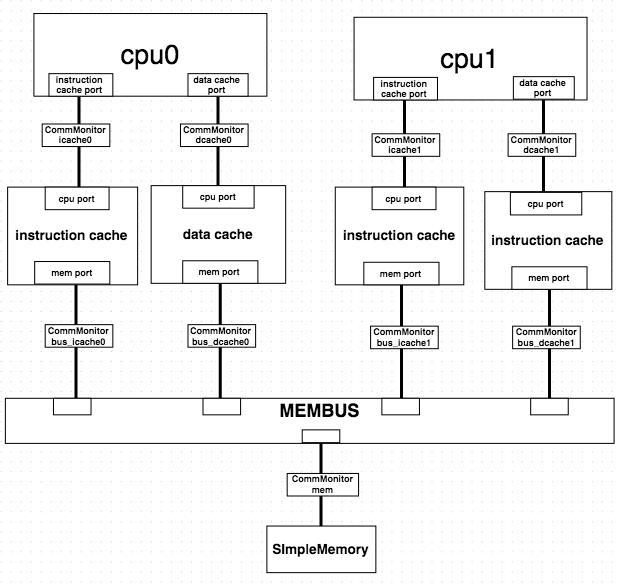
\includegraphics[width=3.3in]{figures/Fig4.png}}
\caption{SoC platform structure.}
\label{SoC}
\end{figure}

In order to find out the efficiency of the trace analysis method for more realistic examples, in this case study, a more detailed transaction level model of a SoC is constructed within the GEM5 environment~\cite{Binkert2011}.  This SoC model consists of two ARM Cortex-A9 cores, each of which contains two separate 16KB data and instruction caches.  The caches are connected to a 1GB memory through a memory bus model.  The architecture of this SoC model is shown in Fig.~\ref{SoC}.  

In this model, components communicate with each other by sending and receiving various request and response messages.  In order to observe and trace communications occurring inside this model during execution, monitors are attached to links connecting the components. These monitors record the messages flowing through the links they are attached to, and store them into output trace files.

%By combining the informations from all of the nine communication monitors, required communication traces are obtained. As a virtualized SoC platform, GEM5 has three types of request: timing, atomic and functional. Timing request include the modeling of queuing delay and resource contention. Atomic request is a faster than timing request with no delay.  Functional request is used for loading binaries, examining/changing variables in the simulated system, and so on. In our case, we specify all our request to be timed as it's the most detailed one.However, some of the system initiation is still atomic and it's not related to our research, so we only took the messages that are timing request from our collected data. 


%\subsection{Flow Specification}

For this model, we consider the flow specifications describing the cache coherence protocols supported in GEM5 that is used to build the model in Fig~\ref{SoC}.  These flow specifications describe data/instruction read operations and data write operations initiated from CPUs.  Three such flows describe the cache coherent protocols for each CPU.  As there are two CPUs in this model, there are actually six such flows considered for this model.  More detailed information about these protocols and the flow specifications can be found online\footnote{\url{https://github.com/cao2/paper/blob/master/Flow\%20Specification.pdf}} to meet the page limit.


%In the following section, a brief overview for the implemented instances of these flows are given. These flow specifications capture how messages are exchanged for different use cases. In this model, a message is defined with the following format, (Src,Dest,Cmd), where Src and Dest refer to the source and destination components of messages, Cmd refers to the operations that the destination component should perform. 
%\begin{figure} 
%\centerline{
%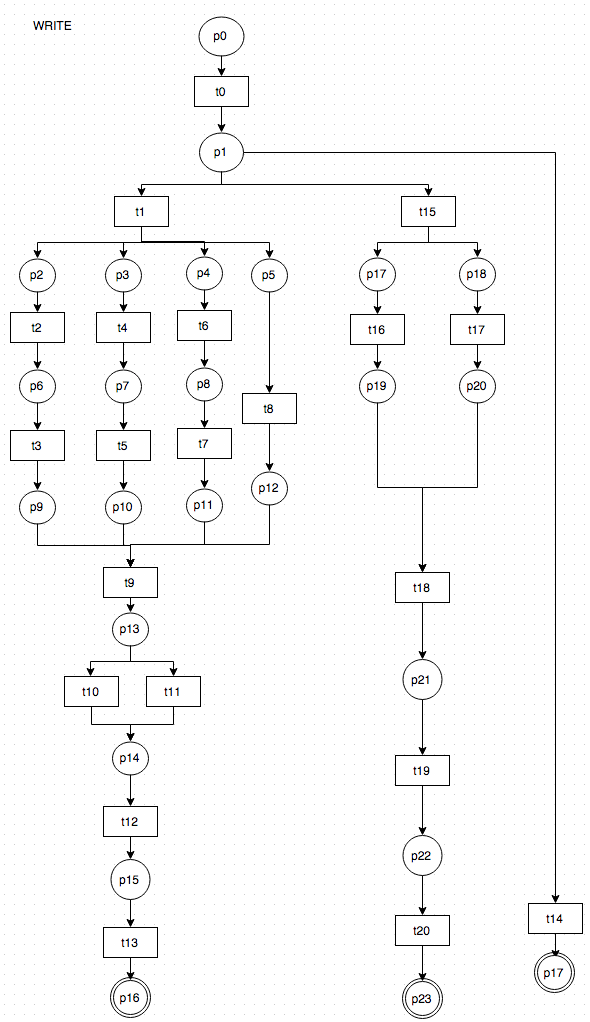
\includegraphics[width=3.7In]{figures/Fig5.png}}
%
%{\footnotesize
%\[
%\begin{array}{llll}
%msg_0: (&\mbox{ CPU1},&\mbox{writeReq},&\mbox{cache1   })\\       
%msg_1: (&\mbox{ cache1},&\mbox{ readExreq },&\mbox{Bus     })\\        
%msg_2: (&\mbox{ Bus},&\mbox{ readExreq},&\mbox{ cahce2 })\\  
%msg_3: (&\mbox{ cache2},&\mbox{readExreq},&\mbox{cpu2         })\\   
%msg_4: (&\mbox{ Bus},&\mbox{ readExreq},&\mbox{ cahce2           })\\  
%msg_5: (&\mbox{ cache2},&\mbox{readExreq},&\mbox{cpu2 })\\  
%msg_6: (&\mbox{ Bus},&\mbox{ readExreq},&\mbox{ cahce1       })\\     
%msg_7: (&\mbox{ cache1},&\mbox{readExreq},&\mbox{cpu1           })\\  
%msg_8: (&\mbox{ Bus},&\mbox{ readExreq},&\mbox{ Memory })\\  
%msg_9: (&\mbox{ true                                          })\\  
%msg_{10}: (&\mbox{ Memory},&\mbox{ readExres},&\mbox{ Bus        })\\  
%msg_{11}: (&\mbox{ cache2},&\mbox{ readExres},&\mbox{ Bus })\\  
%msg_{12}: (&\mbox{ Bus},&\mbox{ readExres},&\mbox{ cache1        })\\  
%msg_{13}: (&\mbox{ cache1},&\mbox{ writeRes},&\mbox{ CPU1         })\\  
%msg_{14}: (&\mbox{ cache1},&\mbox{ writeRes},&\mbox{ CPU1 })\\  
%msg_{15}: (&\mbox{ cache1},&\mbox{UpgradeReq             })\\  
%msg_{16}: (&\mbox{ Bus},&\mbox{ UpgradeReq},&\mbox{ cahce2      })\\   
%msg_{17}: (&\mbox{ Bus},&\mbox{ UpgradeReq},&\mbox{ Memory })\\  
%msg_{18}: (&\mbox{ cache2},&\mbox{UpgradeRes},&\mbox{ Bus     })\\  
%msg_{19}: (&\mbox{ Bus},&\mbox{ UpgradeRes},&\mbox{ cache1      })\\  
%msg_{20}: (&\mbox{ cache1},&\mbox{ WriteRes},&\mbox{ CPU1 })\\  
%\end{array}
%\]}
%\caption{Flow specification ($F_1$) of a cache coherent write operation initiated from CPU1}
%\label{write-flow}
%\end{figure}
%
%The LPN as shown in Fig.~\ref{write-flow} specifies a system flow where CPU1 initiates a memory write operation. In this flow, CPU1 initiates a memory write request to L1 Cache. Next, depends on whether the required data is included in cache1, the cache1 will generate three possible responses. First, the cache1 will send read exclusive request message msg2 to interconnect if data is not present in cache.; Or if the data is shared by CPU0, it will send upgrade message msg16 to interconnect to disable CPU0's ownership of this block of data, else if CPU1 has exclusive right of required data, cache1 will perform the write operation and sent an response message msg15 to CPU1. Afterwards, interconnect will sent request to all connected component (data cache and instruction cache of each CPU and memory). Once the interconnect obtains the response from either CPU0 or memory, it will generate a response message to cache1, then cache1 will generate a write response message msg14 (or msg 21 ) to CPU1. The flow is symmetric for CPU2.
%
%
%\begin{figure} 
%\centerline{
%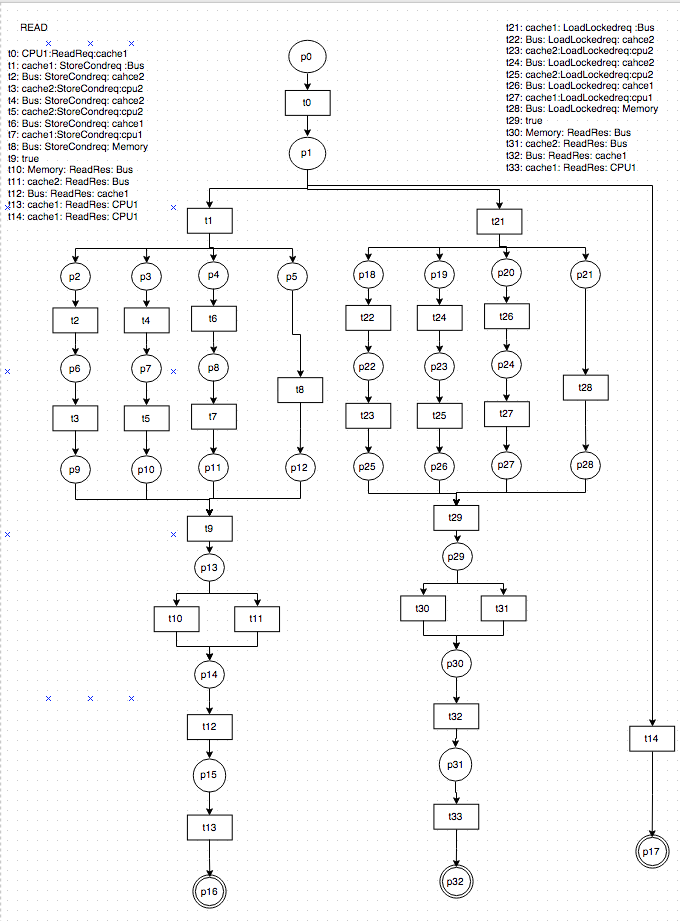
\includegraphics[width=4in]{figures/Fih6.png}}
%
%{\footnotesize
%\[
%\begin{array}{llll}
%t0: (&\mbox{ CPU1},&\mbox{ReadReq},&\mbox{cache1  })\\                   
%t1: (&\mbox{ cache1},&\mbox{ StoreCondreq },&\mbox{Bus })\\           
%t2: (&\mbox{ Bus},&\mbox{ StoreCondreq},&\mbox{ cahce2 })\\
%t3: (&\mbox{ cache2},&\mbox{StoreCondreq},&\mbox{cpu2       })\\      
%t4: (&\mbox{ Bus},&\mbox{ StoreCondreq},&\mbox{ cahce2           })\\ 
%t5: (&\mbox{ cache2},&\mbox{StoreCondreq},&\mbox{cpu2 })\\
%t6: (&\mbox{ Bus},&\mbox{ StoreCondreq},&\mbox{ cahce1     })\\       
%t7: (&\mbox{ cache1},&\mbox{StoreCondreq},&\mbox{cpu1           })\\ 
%t8: (&\mbox{ Bus},&\mbox{ StoreCondreq},&\mbox{ Memory })\\
%t9: (&\mbox{ true                                        })\\
%t10: (&\mbox{ Memory},&\mbox{ ReadRes},&\mbox{ Bus            })\\    
%t11: (&\mbox{ cache2},&\mbox{ ReadRes},&\mbox{ Bus })\\
%t12: (&\mbox{ Bus},&\mbox{ ReadRes},&\mbox{ cache1      })\\            
%t13: (&\mbox{ cache1},&\mbox{ ReadRes},&\mbox{ CPU1          })\\  
%t14: (&\mbox{ cache1},&\mbox{ ReadRes},&\mbox{ CPU1 })\\
%t21: (&\mbox{ cache1},&\mbox{ LoadLockedreq },&\mbox{Bus })\\     
%t22: (&\mbox{ Bus},&\mbox{ LoadLockedreq},&\mbox{ cahce2     })\\
%t23: (&\mbox{ cache2},&\mbox{LoadLockedreq},&\mbox{cpu2 })\\
%t24: (&\mbox{ Bus},&\mbox{ LoadLockedreq},&\mbox{ cahce2     })\\ 
%t25: (&\mbox{ cache2},&\mbox{LoadLockedreq},&\mbox{cpu2     })\\
%t26: (&\mbox{ Bus},&\mbox{ LoadLockedreq},&\mbox{ cahce1 })\\
%t27: (&\mbox{ cache1},&\mbox{LoadLockedreq},&\mbox{cpu1       })\\
%t28: (&\mbox{ Bus},&\mbox{ LoadLockedreq},&\mbox{ Memory     })\\
%t29: (&\mbox{ true })\\
%t30: (&\mbox{ Memory},&\mbox{ ReadRes},&\mbox{ Bus       })\\     
%t31: (&\mbox{ cache2},&\mbox{ ReadRes},&\mbox{ Bus    })\\
%t32: (&\mbox{ Bus},&\mbox{ ReadRes},&\mbox{ cache1 })\\
%t33: (&\mbox{ cache1},&\mbox{ ReadRes},&\mbox{ CPU1 })\\
%\end{array}
%\]}
%\caption{Flow specification ($F_2$) of a cache coherent read operation initiated from CPU1}
%\label{read-flow}
%
%\end{figure}
%The LPN specification as shown in Fig.~\ref{read-flow} captures the system flow where CPU1 initiate a memory read operation. Similar to memory write, CPU1 will first initiate a memory read request message msg1 to cache1. Cache1 can generate three possible responses. First, if the requested data is not in cache1, cache1 will generate an storeCondReq message msg2 to interconnect asking for data. Second, if the requested data is inside of cache1 but it's shared, cache1 will generate a upgrade request message msg22 to make sure it has the newest data; Last,  if cache1 has and data and it's not shared, it will generate a read response message msg15 to CPU1. Afterwards, interconnect will send corresponding request to all of its connected components. When interconnect receives the response, it will generate response message to cache1. Then cache1 will generate the read response message msg14 or msg34 to CPU1. This specification is also symmetric for CPU2.

%%%%%%%%%%%%%%%%%%%%%%%%%%%%%%%%%%%%%%%%%%%%%%%%%%%%%%%%%%%%%%%%%%%%%%
%\subsection{Results and Discussions}

Two simple programs are written, one for each CPU.  These simple programs read numbers from a file, perform some operations on these numbers, and store the results back to the file.  How GEM5 supports shared memory multi-threaded program execution is unclear.  Therefore, there is no data shared in both caches in this test.  Furthermore, GEM5 does not support true concurrency.  When there are two programs running on the CPUs, GEM5 alternates the executions between the two CPUs.  To simulate asynchronous concurrency with the interleaving semantics, those two simple programs are instrumented with pseudo-blocking commands, one placed before each statement.  A pseudo blocking command includes a random number generator that returns either $0$ or $1$ and a loop that only exits when the returned random number is $0$.  

%We produce a result file including all of the communication messages between every components from two simple programs running simultaneously on each CPU.  The program assigned to CPU1 read one file three times for one letter and writing one letter for three times to the same file. CPU2's program will do the same read and write functionalities to the same file, only difference is that CPU2 will write first and then read. One thing we should know about GEM5 is that even when we run these two programs concurrently, it will attempt to produce a concurrent result. The data we collected shows that it's not the real nondeterministic concurrency. What GEM5 did was it allowed two CPUs to execute its own instruction in turn, therefore the order was deterministic. Therefore, no matter how many times we ran the program, it produced the same result. We tried other virtual SoC platform softwares, and this was the best nondeterministic concurrency we can get. Even if this is slightly off with what the real chip should work, it still surve our purpose of testing the correctness of our algorithm.

After the SoC model finishes executing the program, there are totally $343581$ messages collected in the trace file.  Not all of the messages are relevant to the flow specification as many are used by GEM5 to initialize its simulation environment.  After removing those irrelevant messages, the number of messages in the trace file is to reduced to $121138$. 

The time taken to remove the irrelevant messages from the trace is negligible.  The total runtime and the peak memory usage for the trace analysis algorithm to finish the reduced trace are 3 seconds and 12MB, respectively.  From the trace, Table~\ref{table-case-2} shows the number of instances extracted for the six flows describing cache coherent read/write operations initiated from both CPUs. 
\begin{table}[tb]
\caption{The number of flow instances derived by the trace analysis with the full observability.}
\begin{center}
\begin{tabular}{|l|c|}
\hline
Flows & $\#$Instances \\
\hline
\hline
CPU1 Data Read			&  $17582$\\
CPU1 Instruction Read		&  $4002$\\
CPU1 Write				&  $3370$\\
\hline
CPU2 Data Read			&  $17386$\\
CPU2 Instruction Read		&  $3955$\\
CPU2 Write				&  $3308$\\
\hline
\end{tabular}
\end{center}
\label{table-case-2}
\end{table}%

To take the partial observability into account, the four monitors attached to the links between two CPUs and their caches are disabled. Then, the trace is generated by the remaining five monitors from the SoC model executing the same program. After removing all non-observable messages, the trace only contains 15089 messages. The numbers of the flow instances extracted by the trace analysis method are shown in Table~\ref{table-par-obs}.  From these results, the numbers of the flow instances are dropped significantly compared to the results extracted from the trace with the full observability as shown in Table~\ref{table-case-2}. This difference is due to that some communications occurred in the system when executing the program involve the CPUs and their corresponding caches only, and the traffic on the links between the CPUs and their corresponding caches is not observable. Therefore, the instances of the flow specifications characterizing these communications do not exist in the trace. In other words, all extracted flow instances in Table~\ref{table-par-obs} characterize the communications that pass through the memory bus in the system model.  The runtime and memory usage is similar to that for analyzing the trace of the full observability as shown above.

\begin{table}[tb]
\caption{The number of flow instances derived by the trace analysis with certain monitors disabled.}
\begin{center}
\begin{tabular}{|l|c|}
\hline
Flows & $\#$Instances \\
\hline
\hline
CPU1 Data Read			&  $829$\\
CPU1 Instruction Read		&  $169$\\
CPU1 Write				&  $82$\\
\hline
CPU2 Data Read			&  $803$\\
CPU2 Instruction Read		&  $190$\\
CPU2 Write				&  $83$\\
\hline
\end{tabular}
\end{center}
\label{table-par-obs}
\end{table}%

In the third experiment, further partial observability is taken into consideration.  In this experiment, only the five links involving the memory bus are still considered.  However, an assumption is made that all messages passing the same link are not distinguishable due to the limitation of the observability.  More specifically, the monitors are modified such that whenever a message is captured on one of the links, it dumps a set of messages passing through the same link into the trace file.  Therefore, each line of the trace file corresponds to a set of messages.  After applying the trace analysis to this trace,  a total of 13944 flow execution scenarios are extracted.    This large number, compared to the number of extracted execution scenarios shown in the Table~\ref{table-case-2} and \ref{table-par-obs}, is due to the ambiguous interpretation of the messages with limited observability.  

The whole experiment takes about $15$ minutes and $420$~MB to finish, significantly higher than the numbers for analyzing traces where there is no ambiguity in the observed messages.  This is due to the fact that a trace of ambiguous events is in fact a set of traces of original messages, which lead to large numbers of execution scenarios either during or at the end of the analysis.  In this experiment, the peak number of executions during the analysis process is $70384$.   Compared to the final number, many of the intermediate scenarios are invalid, and removed eventually.  However, controlling the number of intermediate scenarios during the trace analysis is critical in order for the analysis to be tractable.  Here, insights from validators can help.    



%=====
\section{Related Work}

Our work is closely related to communication-centric and transaction based debug.  An early pioneering work is described in~\cite{Goossens2007NOCS}, which advocates the focus on observing activities on the interconnect network among IP blocks, and mapping these activities to transactions for better correlation between computations and communications.  Therefore, the communication transactions, as a result of software execution, provide an interface between computation and communication, and facilitate  system-level debug.  This work is extended in~\cite{Vermeulen2009VLSI-DAT,Goossens2009DATE}.  However, this line of work is focused on the network-on-chip (NoC) architecture for interconnect using the run/stop debug control method.  

A similar transaction-based debug approach is presented in~\cite{Gharehbaghi2012ISQED}.  Furthermore, it proposes an automated extraction of state machines at transaction level from  high level design models.  From an observed failure trace, it performs backtracking on this transaction level state machine to derive a set of transaction traces that lead to the observed failure state.  In the subsequent step, bounded model checking with the constraints on the internal variables is used to refine the set of transaction traces to remove the infeasible traces.  This approach requires user inputs to identify impossible transaction sequences, and may not find the states causing the failure if the transaction traces leading to the observed failure state is long.  Backtracking from the observed failure state requires pre-image computation, which can be computationally expensive.  A transaction-based online debug approach is proposed in~\cite{Dehbash2014} to address these issues.  This approach utilizes a transaction debug pattern specification language~\cite{Gharehbaghi2009ICCD} to define properties that transactions should meet.  These transaction properties are checked at runtime by programming debug units in the on-chip debug infrastructure, and the system can be stopped shortly after a violation is detected for any one of those properties.  In this sense, it can be viewed as the hardware assertion approaches in~\cite{Boule2007ISQED} elevated to the transaction level. 

In~\cite{Singerman2011DAC}, a coherent workflow is described where the result from the pre-silicon validation stage can be carried over to the post-silicon stage to improve efficiency and productivity of post-silicon debug.  This workflow is centered on a repository of system events and simple transactions defined by architects and IP designers.  It spans across a wide spectrum of the post-silicon validation including DFx instrumentation, test generation, coverage, and debug.  The DFx instruments are automatically inserted into the design RTL code driven by the defined transactions.  This instrumentation is optimized for making a large set of events and transactions observable.   Test generation is also optimized to generate only the necessary but sufficient tests to allow all defined transactions to be exercised.   Moreover, coverage for post-silicon validation is now defined at the abstract level of events and transactions rather than the raw signals, and thus can be evaluated more efficiently.  In~\cite{Abarbanel2014DAC}, a model at an even higher-level of abstraction, {\em flows}, is proposed.  Flows are used to specify more sophisticated cross-IP transactions such as power management, security, etc, and to facilitate reuse of the efforts of the architectural analysis to check HW/SW implementations. 


%
%--
\section{Conclusion}

This paper presents a trace analysis based method for post-silicon validation by interpreting observed raw signal traces at the level of system flow specifications.  The derived flow execution scenarios provide more structured information on system operations, which is more understandable to system validators.   This information can help to locate design defects more easily, and also provides a measurement of validation coverage.  

Due to partial observability, this approach may derive a large number of different flow execution scenarios for a given signal trace.  Insights from system validators can help to eliminate some false scenarios due to the partial observability.  An interesting future direction is formalization of the validators' insights using temporal logic on flows so that the validators can express their intents more precisely and concisely. 

The trace analysis approach presented in this paper needs to be iterated with different observations selected in different iterations in order to eliminate the false scenarios and to root cause system failures as quickly as possible.  The observation selection and stitching signal traces of different observations together for the above goal will also be pursued in the future.




% conference papers do not normally have an appendix


% use section* for acknowledgement
%\section*{Acknowledgment}
%
%
%The authors would like to thank...
%




% trigger a \newpage just before the given reference
% number - used to balance the columns on the last page
% adjust value as needed - may need to be readjusted if
% the document is modified later
%\IEEEtriggeratref{8}
% The "triggered" command can be changed if desired:
%\IEEEtriggercmd{\enlargethispage{-5in}}

% references section

% can use a bibliography generated by BibTeX as a .bbl file
% BibTeX documentation can be easily obtained at:
% http://www.ctan.org/tex-archive/biblio/bibtex/contrib/doc/
% The IEEEtran BibTeX style support page is at:
% http://www.michaelshell.org/tex/ieeetran/bibtex/
\bibliographystyle{IEEEtran}
% argument is your BibTeX string definitions and bibliography database(s)
\bibliography{SoC}
%
% <OR> manually copy in the resultant .bbl file
% set second argument of \begin to the number of references
% (used to reserve space for the reference number labels box)
%\begin{thebibliography}{1}
%
%\bibitem{IEEEhowto:kopka}
%H.~Kopka and P.~W. Daly, \emph{A Guide to \LaTeX}, 3rd~ed.\hskip 1em plus
%  0.5em minus 0.4em\relax Harlow, England: Addison-Wesley, 1999.
%
%\end{thebibliography}




% that's all folks
\end{document}


